\makeatletter \@ifundefined{rootpath}{% Manual to memoir http://mirrors.dotsrc.org/ctan/macros/latex/contrib/memoir/memman.pdf

%\documentclass[a4paper,12pt,fleqn,openany,twoside]{memoir} %two sides for printing
\documentclass[a4paper,12pt,fleqn,openany,oneside]{memoir} %one side for pdf
\usepackage[english]{babel}
\usepackage[utf8]{inputenc}
\usepackage{microtype}
\usepackage{paralist}

%Definitions
\usepackage{amsthm}
\theoremstyle{plain}
\newtheorem{thm}{Theorem}[chapter] % reset theorem numbering for each chapter
\theoremstyle{definition}
\newtheorem{defn}[thm]{Definition}


% Choses the depth of numerations
\setsecnumdepth{subsubsection}

% Choses the depth of toc
%\maxtocdepth{subsection}

% LaTeX logical statements
\usepackage{ifthen}

% Fancy space after use of e.g. command
\usepackage{xspace}

% Skips after paragraphs
\usepackage{parskip}

% Layout settings
\setlength{\parindent}{0cm}
\setlength{\parskip}{2ex plus 2ex} %kan udvides til f.eks: '2ex plus 2ex minus 0ex'

\sloppybottom

% Don't make a collection per default
\newcommand{\worksheetcollection}{false}

% Bibtex
\usepackage[square,numbers,sort,comma]{natbib}
%\usepackage{cite}
%\bibliographystyle{plainnat}
\bibliographystyle{IEEEtran}


% Fixmes
\usepackage{fixme}
\fxsetup{draft}

% Mathematic
\usepackage{amsmath}
\usepackage{amsfonts}
\usepackage{amssymb}
\usepackage{stmaryrd}
\allowdisplaybreaks[1]


% Acronyms
\usepackage[printonlyused]{acronym}

% Images
\usepackage{graphicx}
\usepackage{wrapfig}
\usepackage[outdir=./]{epstopdf}
\usepackage{epsfig}


% Captions ans subcaptions
\captionnamefont{\footnotesize\bfseries}
\captiontitlefont{\footnotesize}

% Enable memoir subfloats for figures and tables
\newsubfloat{figure}
\newsubfloat{table}

% Hack memoir subfigure styles to have bold label and footnotesize fonts
\renewcommand{\thesubfigure}{\footnotesize\bfseries{(\alph{subfigure})}}
\renewcommand{\thesubtable}{\footnotesize\bfseries{(\alph{subtable})}}

\renewcommand{\subcaption}[2][]{\subbottom[\footnotesize{#1}]{#2}}

% Memoir tweak pagenumbers
%\pagestyle{headings}

% Tikz
\usepackage{tikz}
\usetikzlibrary{arrows,shapes,calc,positioning}
\pgfmathsetseed{1}

%Pgf plots
\usepackage{pgfplots}
\pgfplotsset{compat=1.5}
% loatbarrier, keep figures within (sub,subsub) sections
\usepackage{placeins}
\usepackage{pgfplots}
\usepgfplotslibrary{units}
\usepackage[space-before-unit,range-units = repeat]{siunitx}

% Hyperlinked auto references
\usepackage[hidelinks]{hyperref}
\usepackage[nameinlink]{cleveref}
\crefname{lstlisting}{Listing}{Listings}  
\Crefname{lstlisting}{Listing}{Listings}

\crefname{thm}{definition}{definitions}
\Crefname{thm}{Definition}{Definitions}

%\def\chapterautorefname{Kapitel}
%\def\sectionautorefname{Afsnit}
%\def\subsectionautorefname{Afsnit}
%\def\subsubsectionautorefname{Underafsnit}
%\def\figureautorefname{Figur}
%\def\lstlistingautorefname{Listing}
%\def\lstnumberautorefname{Linje}
%\def\itemautorefname{Punkt}
\usepackage[hypcap]{caption} % Link to top of the figure and not the caption

%Sick shit to make \Autoref command
%http://tex.stackexchange.com/questions/36575/autorefs-inserted-text-has-not-the-correct-case
\def\HyLang@english{%
  \def\equationautorefname{Equation}%
  \def\footnoteautorefname{Footnote}%
  \def\itemautorefname{item}%
  \def\figureautorefname{Figure}%
  \def\tableautorefname{Table}%
  \def\partautorefname{Part}%
  \def\appendixautorefname{Appendix}%
  \def\chapterautorefname{Chapter}%
  \def\sectionautorefname{Section}%
  \def\subsectionautorefname{Subsection}%
  \def\subsubsectionautorefname{Subsubsection}%
  \def\paragraphautorefname{Paragraph}%
  \def\subparagraphautorefname{Subparagraph}%
  \def\FancyVerbLineautorefname{Line}%
  \def\theoremautorefname{Theorem}%
  \def\pageautorefname{Page}%
}

% Reference greencommentssections with number and name
\usepackage{nameref}
\newcommand{\bsnameref}[1]{\Cref{#1} ``\nameref{#1}''}
\newcommand{\bsref}[1]{\Cref{#1}}
\newcommand{\bsbilagref}[1]{Appendix \ref{#1}}
\newcommand{\bsbilagnameref}[1]{Appendix \ref{#1} ``\nameref{#1}''}
\newcommand{\pling}[1]{``#1''}


% Listings for code qoutes
\usepackage{listings}
%\usepackage[usenames,dvipsnames,svgnames,table]{xcolor}
\usepackage{color}
\usepackage{xcolor}
\definecolor{bluekeywords}{rgb}{0.13,0.13,1}
\definecolor{greencomments}{rgb}{0,0.5,0}
\definecolor{redstrings}{rgb}{0.9,0,0}
\usepackage{caption} 
\usepackage{multicol}
\DeclareCaptionFont{white}{\color{white}}
\DeclareCaptionFormat{listing}{\colorbox{gray}{\parbox{\textwidth}{#1#2#3}}}
\captionsetup[lstlisting]{format=listing,labelfont=white,textfont=white}
%\lstset{numbers=left}
\lstset{
	basicstyle=\footnotesize,
	tabsize=2,
	breaklines=true,
  literate={æ}{{\ae}}1 {ø}{{\o}}1 {å}{{\aa}}1 {Æ}{{\AE}}1 {Ø}{{\O}}1 {Å}{{\AA}}1,
  keywords={typeof, new, true, false, catch, function, return, null, catch, switch, var, if, in, while, do, else, case, break},
  keywordstyle=\color{blue}\bfseries,
  ndkeywords={class, export, boolean, throw, implements, import, this},
  ndkeywordstyle=\color{darkgray}\bfseries,
  identifierstyle=\color{black},
  sensitive=false,
  comment=[l]{//},
  morecomment=[s]{/*}{*/},
  commentstyle=\color{purple}\ttfamily,
  stringstyle=\color{red}\ttfamily,
  numbers=left,
  numbersep=-5pt,
  showstringspaces=false,
  showspaces=false,
  %morestring=[b]',
  %morestring=[b]"
}
\lstnewenvironment{code}[1][]%
  {\minipage{\linewidth} 
   \lstset{basicstyle=\ttfamily\footnotesize,frame=single,#1}}
  {\endminipage}

\lstdefinelanguage{scala}{
  morekeywords={abstract,case,catch,class,def,%
    do,else,extends,false,final,finally,%
    for,if,implicit,import,match,mixin,%
    new,null,object,override,package,%
    private,protected,requires,return,sealed,%
    super,this,throw,trait,true,try,%
    type,val,var,while,with,yield, Unit, Boolean, Int},
  otherkeywords={=>,<-,<\%,<:,>:,\#,@},
  sensitive=true,
  morecomment=[l]{//},
  morecomment=[n]{/*}{*/},
  morestring=[b]",
  morestring=[b]',
  morestring=[b]"""
}

\lstdefinelanguage{clojure}%
{morekeywords={*,*1,*2,*3,*agent*,*allow-unresolved-vars*,*assert*,*clojure-version*,*command-line-args*,%
*compile-files*,*compile-path*,*e,*err*,*file*,*flush-on-newline*,*in*,*macro-meta*,%
*math-context*,*ns*,*out*,*print-dup*,*print-length*,*print-level*,*print-meta*,*print-readably*,%
*read-eval*,*source-path*,*use-context-classloader*,*warn-on-reflection*,+,-,->,->>,..,/,:else,%
<,<=,=,==,>,>=,@,accessor,aclone,add-classpath,add-watch,agent,agent-errors,aget,alength,alias,%
all-ns,alter,alter-meta!,alter-var-root,amap,ancestors,and,apply,areduce,array-map,aset,%
aset-boolean,aset-byte,aset-char,aset-double,aset-float,aset-int,aset-long,aset-short,assert,%
assoc,assoc!,assoc-in,associative?,atom,await,await-for,await1,bases,bean,bigdec,bigint,binding,%
bit-and,bit-and-not,bit-clear,bit-flip,bit-not,bit-or,bit-set,bit-shift-left,bit-shift-right,%
bit-test,bit-xor,boolean,boolean-array,booleans,bound-fn,bound-fn*,butlast,byte,byte-array,%
bytes,cast,char,char-array,char-escape-string,char-name-string,char?,chars,chunk,chunk-append,%
chunk-buffer,chunk-cons,chunk-first,chunk-next,chunk-rest,chunked-seq?,class,class?,%
clear-agent-errors,clojure-version,coll?,comment,commute,comp,comparator,compare,compare-and-set!,%
compile,complement,concat,cond,condp,conj,conj!,cons,constantly,construct-proxy,contains?,count,%
counted?,create-ns,create-struct,cycle,dec,decimal?,declare,def,definline,defmacro,defmethod,%
defmulti,defn,defn-,defonce,defprotocol,defstruct,deftype,delay,delay?,deliver,deref,derive,%
descendants,destructure,disj,disj!,dissoc,dissoc!,distinct,distinct?,do,do-template,doall,doc,%
dorun,doseq,dosync,dotimes,doto,double,double-array,doubles,drop,drop-last,drop-while,empty,empty?,%
ensure,enumeration-seq,eval,even?,every?,false,false?,ffirst,file-seq,filter,finally,find,find-doc,%
find-ns,find-var,first,float,float-array,float?,floats,flush,fn,fn?,fnext,for,force,format,future,%
future-call,future-cancel,future-cancelled?,future-done?,future?,gen-class,gen-interface,gensym,%
get,get-in,get-method,get-proxy-class,get-thread-bindings,get-validator,hash,hash-map,hash-set,%
identical?,identity,if,if-let,if-not,ifn?,import,in-ns,inc,init-proxy,instance?,int,int-array,%
integer?,interleave,intern,interpose,into,into-array,ints,io!,isa?,iterate,iterator-seq,juxt,%
key,keys,keyword,keyword?,last,lazy-cat,lazy-seq,let,letfn,line-seq,list,list*,list?,load,load-file,%
load-reader,load-string,loaded-libs,locking,long,long-array,longs,loop,macroexpand,macroexpand-1,%
make-array,make-hierarchy,map,map?,mapcat,max,max-key,memfn,memoize,merge,merge-with,meta,%
method-sig,methods,min,min-key,mod,monitor-enter,monitor-exit,name,namespace,neg?,new,newline,%
next,nfirst,nil,nil?,nnext,not,not-any?,not-empty,not-every?,not=,ns,ns-aliases,ns-imports,%
ns-interns,ns-map,ns-name,ns-publics,ns-refers,ns-resolve,ns-unalias,ns-unmap,nth,nthnext,num,%
number?,odd?,or,parents,partial,partition,pcalls,peek,persistent!,pmap,pop,pop!,pop-thread-bindings,%
pos?,pr,pr-str,prefer-method,prefers,primitives-classnames,print,print-ctor,print-doc,print-dup,%
print-method,print-namespace-doc,print-simple,print-special-doc,print-str,printf,println,println-str,%
prn,prn-str,promise,proxy,proxy-call-with-super,proxy-mappings,proxy-name,proxy-super,%
push-thread-bindings,pvalues,quot,rand,rand-int,range,ratio?,rational?,rationalize,re-find,%
re-groups,re-matcher,re-matches,re-pattern,re-seq,read,read-line,read-string,recur,reduce,ref,%
ref-history-count,ref-max-history,ref-min-history,ref-set,refer,refer-clojure,reify,%
release-pending-sends,rem,remove,remove-method,remove-ns,remove-watch,repeat,repeatedly,%
replace,replicate,require,reset!,reset-meta!,resolve,rest,resultset-seq,reverse,reversible?,%
rseq,rsubseq,second,select-keys,send,send-off,seq,seq?,seque,sequence,sequential?,set,set!,%
set-validator!,set?,short,short-array,shorts,shutdown-agents,slurp,some,sort,sort-by,sorted-map,%
sorted-map-by,sorted-set,sorted-set-by,sorted?,special-form-anchor,special-symbol?,split-at,%
split-with,str,stream?,string?,struct,struct-map,subs,subseq,subvec,supers,swap!,symbol,symbol?,%
sync,syntax-symbol-anchor,take,take-last,take-nth,take-while,test,the-ns,throw,time,to-array,%
to-array-2d,trampoline,transient,tree-seq,true,true?,try,type,unchecked-add,unchecked-dec,%
unchecked-divide,unchecked-inc,unchecked-multiply,unchecked-negate,unchecked-remainder,%
unchecked-subtract,underive,unquote,unquote-splicing,update-in,update-proxy,use,val,vals,%
var,var-get,var-set,var?,vary-meta,vec,vector,vector?,when,when-first,when-let,when-not,%
while,with-bindings,with-bindings*,with-in-str,with-loading-context,with-local-vars,%
with-meta,with-open,with-out-str,with-precision,xml-seq,zero?,zipmap
},%
   sensitive,% ???
   alsodigit=-,%
   morecomment=[l];,%
   morestring=[b]"%
  }[keywords,comments,strings]%

% Worksheet commands
\newcommand{\worksheetstart}[5]{ %Title, Revision, Date, Author, rootpath
	\ifthenelse{\equal{\worksheetcollection}{false}}{
		\newcommand{\rootpath}{#5}
		\documentheader
		\chapter{#1}
	}{
		\chapter{#1}
	}
%	\vspace{-1em}
%	\textbf{\tiny Revision #2 at #3. Written by #4}\\
%	\textbf{\tiny Hovedansvarlig #4}\\
%	\vspace{2em}\\
}

\newcommand{\worksheetend}{
	\ifthenelse{\equal{\worksheetcollection}{false}}{
		\collectionend
	}{}
}

\newcommand{\documentheader}{
	% Draws a tikz camera
% #1 is the coordinate to the top left corner
% #2 is a label for the righthand center position
% #3 is the text shown in the center of the camera
\newcommand{\camera}[3]{
\coordinate (anchor) at #1;
\draw (anchor) -- ($ (anchor) + (0em,-20pt) $) -- ($ (anchor) + (10pt, -15pt) $) -- ($ (anchor) + (10pt,-5pt)$) -- cycle;
\draw ($ (anchor) + (10pt,-5pt) $) -- ($ (anchor) + (10pt,0pt) $) -- ($ (anchor) + (50pt,0pt) $) -- ($ (anchor) + (50pt,-20pt) $) -- node[yshift=10pt] {\tiny #3} ($ (anchor) + (10pt,-20pt) $)-- cycle;
\coordinate (#2) at ($ (anchor) + (50pt,-10pt) $);
}

\newcounter{frameNumber}
\newcommand{\frameWithSize}[3][false]{
	\stepcounter{frameNumber}
	\coordinate (anchor) at #2;
	\ifthenelse{\equal{#1}{false}}{
		\def\frameNumber{\arabic{frameNumber}}
	}{
		\def\frameNumber{#1}
	}
	\pgfmathtruncatemacro\randomnumber{random(0,4)}
	\node[yshift=20pt] at (anchor) {\frameNumber};
	\ifthenelse{\equal{#3}{I}}{
		\node[draw, minimum size=20pt, fill=green!60] at (anchor) {I};
		\filldraw[fill=gray] ($(anchor) + (-10pt,-40pt)$) rectangle ($(anchor) + (10pt,-20pt) + (0pt,\randomnumber pt)$);
	}{
		\ifthenelse{\equal{#3}{P}}{
			\node[draw, minimum size=20pt, fill=yellow!60] at (anchor) {P};
			\filldraw[fill=gray] ($(anchor) + (-10pt,-40pt)$) rectangle ($(anchor) + (10pt,-30pt) + (0pt,\randomnumber pt)$);
		}{
			\node[draw, minimum size=20pt, fill=blue!40!yellow!60!black] at (anchor) {\color{white}B};
			\filldraw[fill=gray] ($(anchor) + (-10pt,-40pt)$) rectangle ($(anchor) + (10pt,-37pt) + (0pt,\randomnumber pt)$);
		}
	}
	\draw[thick] ($(anchor) + (-10pt,-40pt)$) -- +(20pt,0pt);
}

	\begin{document}
	%\renewcommand{\chaptername}{Worksheet}
	\chapterstyle{section}
	\renewcommand{\beforechapskip}{0pt}
	\renewcommand{\afterchapskip}{0pt}
}

\newcommand{\collectionstart}[1]{
	\newcommand{\rootpath}{#1}
	\renewcommand{\worksheetcollection}{true}
	\documentheader
	\frontmatter
	%\forside
	\makeatletter \@ifundefined{rootpath}{% Manual to memoir http://mirrors.dotsrc.org/ctan/macros/latex/contrib/memoir/memman.pdf

%\documentclass[a4paper,12pt,fleqn,openany,twoside]{memoir} %two sides for printing
\documentclass[a4paper,12pt,fleqn,openany,oneside]{memoir} %one side for pdf
\usepackage[english]{babel}
\usepackage[utf8]{inputenc}
\usepackage{microtype}
\usepackage{paralist}

%Definitions
\usepackage{amsthm}
\theoremstyle{plain}
\newtheorem{thm}{Theorem}[chapter] % reset theorem numbering for each chapter
\theoremstyle{definition}
\newtheorem{defn}[thm]{Definition}


% Choses the depth of numerations
\setsecnumdepth{subsubsection}

% Choses the depth of toc
%\maxtocdepth{subsection}

% LaTeX logical statements
\usepackage{ifthen}

% Fancy space after use of e.g. command
\usepackage{xspace}

% Skips after paragraphs
\usepackage{parskip}

% Layout settings
\setlength{\parindent}{0cm}
\setlength{\parskip}{2ex plus 2ex} %kan udvides til f.eks: '2ex plus 2ex minus 0ex'

\sloppybottom

% Don't make a collection per default
\newcommand{\worksheetcollection}{false}

% Bibtex
\usepackage[square,numbers,sort,comma]{natbib}
%\usepackage{cite}
%\bibliographystyle{plainnat}
\bibliographystyle{IEEEtran}


% Fixmes
\usepackage{fixme}
\fxsetup{draft}

% Mathematic
\usepackage{amsmath}
\usepackage{amsfonts}
\usepackage{amssymb}
\usepackage{stmaryrd}
\allowdisplaybreaks[1]


% Acronyms
\usepackage[printonlyused]{acronym}

% Images
\usepackage{graphicx}
\usepackage{wrapfig}
\usepackage[outdir=./]{epstopdf}
\usepackage{epsfig}


% Captions ans subcaptions
\captionnamefont{\footnotesize\bfseries}
\captiontitlefont{\footnotesize}

% Enable memoir subfloats for figures and tables
\newsubfloat{figure}
\newsubfloat{table}

% Hack memoir subfigure styles to have bold label and footnotesize fonts
\renewcommand{\thesubfigure}{\footnotesize\bfseries{(\alph{subfigure})}}
\renewcommand{\thesubtable}{\footnotesize\bfseries{(\alph{subtable})}}

\renewcommand{\subcaption}[2][]{\subbottom[\footnotesize{#1}]{#2}}

% Memoir tweak pagenumbers
%\pagestyle{headings}

% Tikz
\usepackage{tikz}
\usetikzlibrary{arrows,shapes,calc,positioning}
\pgfmathsetseed{1}

%Pgf plots
\usepackage{pgfplots}
\pgfplotsset{compat=1.5}
% loatbarrier, keep figures within (sub,subsub) sections
\usepackage{placeins}
\usepackage{pgfplots}
\usepgfplotslibrary{units}
\usepackage[space-before-unit,range-units = repeat]{siunitx}

% Hyperlinked auto references
\usepackage[hidelinks]{hyperref}
\usepackage[nameinlink]{cleveref}
\crefname{lstlisting}{Listing}{Listings}  
\Crefname{lstlisting}{Listing}{Listings}

\crefname{thm}{definition}{definitions}
\Crefname{thm}{Definition}{Definitions}

%\def\chapterautorefname{Kapitel}
%\def\sectionautorefname{Afsnit}
%\def\subsectionautorefname{Afsnit}
%\def\subsubsectionautorefname{Underafsnit}
%\def\figureautorefname{Figur}
%\def\lstlistingautorefname{Listing}
%\def\lstnumberautorefname{Linje}
%\def\itemautorefname{Punkt}
\usepackage[hypcap]{caption} % Link to top of the figure and not the caption

%Sick shit to make \Autoref command
%http://tex.stackexchange.com/questions/36575/autorefs-inserted-text-has-not-the-correct-case
\def\HyLang@english{%
  \def\equationautorefname{Equation}%
  \def\footnoteautorefname{Footnote}%
  \def\itemautorefname{item}%
  \def\figureautorefname{Figure}%
  \def\tableautorefname{Table}%
  \def\partautorefname{Part}%
  \def\appendixautorefname{Appendix}%
  \def\chapterautorefname{Chapter}%
  \def\sectionautorefname{Section}%
  \def\subsectionautorefname{Subsection}%
  \def\subsubsectionautorefname{Subsubsection}%
  \def\paragraphautorefname{Paragraph}%
  \def\subparagraphautorefname{Subparagraph}%
  \def\FancyVerbLineautorefname{Line}%
  \def\theoremautorefname{Theorem}%
  \def\pageautorefname{Page}%
}

% Reference greencommentssections with number and name
\usepackage{nameref}
\newcommand{\bsnameref}[1]{\Cref{#1} ``\nameref{#1}''}
\newcommand{\bsref}[1]{\Cref{#1}}
\newcommand{\bsbilagref}[1]{Appendix \ref{#1}}
\newcommand{\bsbilagnameref}[1]{Appendix \ref{#1} ``\nameref{#1}''}
\newcommand{\pling}[1]{``#1''}


% Listings for code qoutes
\usepackage{listings}
%\usepackage[usenames,dvipsnames,svgnames,table]{xcolor}
\usepackage{color}
\usepackage{xcolor}
\definecolor{bluekeywords}{rgb}{0.13,0.13,1}
\definecolor{greencomments}{rgb}{0,0.5,0}
\definecolor{redstrings}{rgb}{0.9,0,0}
\usepackage{caption} 
\usepackage{multicol}
\DeclareCaptionFont{white}{\color{white}}
\DeclareCaptionFormat{listing}{\colorbox{gray}{\parbox{\textwidth}{#1#2#3}}}
\captionsetup[lstlisting]{format=listing,labelfont=white,textfont=white}
%\lstset{numbers=left}
\lstset{
	basicstyle=\footnotesize,
	tabsize=2,
	breaklines=true,
  literate={æ}{{\ae}}1 {ø}{{\o}}1 {å}{{\aa}}1 {Æ}{{\AE}}1 {Ø}{{\O}}1 {Å}{{\AA}}1,
  keywords={typeof, new, true, false, catch, function, return, null, catch, switch, var, if, in, while, do, else, case, break},
  keywordstyle=\color{blue}\bfseries,
  ndkeywords={class, export, boolean, throw, implements, import, this},
  ndkeywordstyle=\color{darkgray}\bfseries,
  identifierstyle=\color{black},
  sensitive=false,
  comment=[l]{//},
  morecomment=[s]{/*}{*/},
  commentstyle=\color{purple}\ttfamily,
  stringstyle=\color{red}\ttfamily,
  numbers=left,
  numbersep=-5pt,
  showstringspaces=false,
  showspaces=false,
  %morestring=[b]',
  %morestring=[b]"
}
\lstnewenvironment{code}[1][]%
  {\minipage{\linewidth} 
   \lstset{basicstyle=\ttfamily\footnotesize,frame=single,#1}}
  {\endminipage}

\lstdefinelanguage{scala}{
  morekeywords={abstract,case,catch,class,def,%
    do,else,extends,false,final,finally,%
    for,if,implicit,import,match,mixin,%
    new,null,object,override,package,%
    private,protected,requires,return,sealed,%
    super,this,throw,trait,true,try,%
    type,val,var,while,with,yield, Unit, Boolean, Int},
  otherkeywords={=>,<-,<\%,<:,>:,\#,@},
  sensitive=true,
  morecomment=[l]{//},
  morecomment=[n]{/*}{*/},
  morestring=[b]",
  morestring=[b]',
  morestring=[b]"""
}

\lstdefinelanguage{clojure}%
{morekeywords={*,*1,*2,*3,*agent*,*allow-unresolved-vars*,*assert*,*clojure-version*,*command-line-args*,%
*compile-files*,*compile-path*,*e,*err*,*file*,*flush-on-newline*,*in*,*macro-meta*,%
*math-context*,*ns*,*out*,*print-dup*,*print-length*,*print-level*,*print-meta*,*print-readably*,%
*read-eval*,*source-path*,*use-context-classloader*,*warn-on-reflection*,+,-,->,->>,..,/,:else,%
<,<=,=,==,>,>=,@,accessor,aclone,add-classpath,add-watch,agent,agent-errors,aget,alength,alias,%
all-ns,alter,alter-meta!,alter-var-root,amap,ancestors,and,apply,areduce,array-map,aset,%
aset-boolean,aset-byte,aset-char,aset-double,aset-float,aset-int,aset-long,aset-short,assert,%
assoc,assoc!,assoc-in,associative?,atom,await,await-for,await1,bases,bean,bigdec,bigint,binding,%
bit-and,bit-and-not,bit-clear,bit-flip,bit-not,bit-or,bit-set,bit-shift-left,bit-shift-right,%
bit-test,bit-xor,boolean,boolean-array,booleans,bound-fn,bound-fn*,butlast,byte,byte-array,%
bytes,cast,char,char-array,char-escape-string,char-name-string,char?,chars,chunk,chunk-append,%
chunk-buffer,chunk-cons,chunk-first,chunk-next,chunk-rest,chunked-seq?,class,class?,%
clear-agent-errors,clojure-version,coll?,comment,commute,comp,comparator,compare,compare-and-set!,%
compile,complement,concat,cond,condp,conj,conj!,cons,constantly,construct-proxy,contains?,count,%
counted?,create-ns,create-struct,cycle,dec,decimal?,declare,def,definline,defmacro,defmethod,%
defmulti,defn,defn-,defonce,defprotocol,defstruct,deftype,delay,delay?,deliver,deref,derive,%
descendants,destructure,disj,disj!,dissoc,dissoc!,distinct,distinct?,do,do-template,doall,doc,%
dorun,doseq,dosync,dotimes,doto,double,double-array,doubles,drop,drop-last,drop-while,empty,empty?,%
ensure,enumeration-seq,eval,even?,every?,false,false?,ffirst,file-seq,filter,finally,find,find-doc,%
find-ns,find-var,first,float,float-array,float?,floats,flush,fn,fn?,fnext,for,force,format,future,%
future-call,future-cancel,future-cancelled?,future-done?,future?,gen-class,gen-interface,gensym,%
get,get-in,get-method,get-proxy-class,get-thread-bindings,get-validator,hash,hash-map,hash-set,%
identical?,identity,if,if-let,if-not,ifn?,import,in-ns,inc,init-proxy,instance?,int,int-array,%
integer?,interleave,intern,interpose,into,into-array,ints,io!,isa?,iterate,iterator-seq,juxt,%
key,keys,keyword,keyword?,last,lazy-cat,lazy-seq,let,letfn,line-seq,list,list*,list?,load,load-file,%
load-reader,load-string,loaded-libs,locking,long,long-array,longs,loop,macroexpand,macroexpand-1,%
make-array,make-hierarchy,map,map?,mapcat,max,max-key,memfn,memoize,merge,merge-with,meta,%
method-sig,methods,min,min-key,mod,monitor-enter,monitor-exit,name,namespace,neg?,new,newline,%
next,nfirst,nil,nil?,nnext,not,not-any?,not-empty,not-every?,not=,ns,ns-aliases,ns-imports,%
ns-interns,ns-map,ns-name,ns-publics,ns-refers,ns-resolve,ns-unalias,ns-unmap,nth,nthnext,num,%
number?,odd?,or,parents,partial,partition,pcalls,peek,persistent!,pmap,pop,pop!,pop-thread-bindings,%
pos?,pr,pr-str,prefer-method,prefers,primitives-classnames,print,print-ctor,print-doc,print-dup,%
print-method,print-namespace-doc,print-simple,print-special-doc,print-str,printf,println,println-str,%
prn,prn-str,promise,proxy,proxy-call-with-super,proxy-mappings,proxy-name,proxy-super,%
push-thread-bindings,pvalues,quot,rand,rand-int,range,ratio?,rational?,rationalize,re-find,%
re-groups,re-matcher,re-matches,re-pattern,re-seq,read,read-line,read-string,recur,reduce,ref,%
ref-history-count,ref-max-history,ref-min-history,ref-set,refer,refer-clojure,reify,%
release-pending-sends,rem,remove,remove-method,remove-ns,remove-watch,repeat,repeatedly,%
replace,replicate,require,reset!,reset-meta!,resolve,rest,resultset-seq,reverse,reversible?,%
rseq,rsubseq,second,select-keys,send,send-off,seq,seq?,seque,sequence,sequential?,set,set!,%
set-validator!,set?,short,short-array,shorts,shutdown-agents,slurp,some,sort,sort-by,sorted-map,%
sorted-map-by,sorted-set,sorted-set-by,sorted?,special-form-anchor,special-symbol?,split-at,%
split-with,str,stream?,string?,struct,struct-map,subs,subseq,subvec,supers,swap!,symbol,symbol?,%
sync,syntax-symbol-anchor,take,take-last,take-nth,take-while,test,the-ns,throw,time,to-array,%
to-array-2d,trampoline,transient,tree-seq,true,true?,try,type,unchecked-add,unchecked-dec,%
unchecked-divide,unchecked-inc,unchecked-multiply,unchecked-negate,unchecked-remainder,%
unchecked-subtract,underive,unquote,unquote-splicing,update-in,update-proxy,use,val,vals,%
var,var-get,var-set,var?,vary-meta,vec,vector,vector?,when,when-first,when-let,when-not,%
while,with-bindings,with-bindings*,with-in-str,with-loading-context,with-local-vars,%
with-meta,with-open,with-out-str,with-precision,xml-seq,zero?,zipmap
},%
   sensitive,% ???
   alsodigit=-,%
   morecomment=[l];,%
   morestring=[b]"%
  }[keywords,comments,strings]%

% Worksheet commands
\newcommand{\worksheetstart}[5]{ %Title, Revision, Date, Author, rootpath
	\ifthenelse{\equal{\worksheetcollection}{false}}{
		\newcommand{\rootpath}{#5}
		\documentheader
		\chapter{#1}
	}{
		\chapter{#1}
	}
%	\vspace{-1em}
%	\textbf{\tiny Revision #2 at #3. Written by #4}\\
%	\textbf{\tiny Hovedansvarlig #4}\\
%	\vspace{2em}\\
}

\newcommand{\worksheetend}{
	\ifthenelse{\equal{\worksheetcollection}{false}}{
		\collectionend
	}{}
}

\newcommand{\documentheader}{
	\input{\rootpath/setup/tikz-commands.tex}
	\begin{document}
	%\renewcommand{\chaptername}{Worksheet}
	\chapterstyle{section}
	\renewcommand{\beforechapskip}{0pt}
	\renewcommand{\afterchapskip}{0pt}
}

\newcommand{\collectionstart}[1]{
	\newcommand{\rootpath}{#1}
	\renewcommand{\worksheetcollection}{true}
	\documentheader
	\frontmatter
	%\forside
	\input{\rootpath/worksheets/titlepage/titlepage}
	\input{\rootpath/worksheets/preface/preface}
	%\input{\rootpath/worksheets/forord/forord}
	\newpage
	\newpage
	\tableofcontents*
	\mainmatter
}

\newcommand{\collectionend}{
	\backmatter
	\chapter{List of Acronyms}\vspace{3em}
	\input{\rootpath/setup/acronyms}
	\bibliography{\rootpath/setup/bibliography}
	\end{document}
}


\newcommand{\bscode}{
	\lstinline
}

\newcommand{\bscodemath}[1]{
	\text{\lstinline|#1|}
}

\newcommand{\bsqoute}[2]{
	\begin{quote}
		\textit{``#1''}
		\begin{center}
			-- \emph{#2}
		\end{center}
	\end{quote}
}


\newcommand{\lag}{\langle}
\newcommand{\rag}{\rangle}
\newcommand{\besk}[1]{\ensuremath{\lag #1 \rag}}

\newcommand{\namedtodo}[5]
{
  \ifthenelse{\equal{#1}{}}
  {
    \todo[color=#4,caption=
    {\textbf{#3: } #2}]
    {\color{#5}\textbf{#3: }#2}
  }
  {
    \todo[color=#4,caption=
    {\textbf{#3: } #1}
    ,inline]
    {\color{#5}\textbf{#3: }#2}
  }
}
\newcommand{\andreas}[2][]{\namedtodo{#1}{#2}{Andreas}{blue!50!red!10}{black}}
\newcommand{\lone}[2][]{\namedtodo{#1}{#2}{Lone}{orange}{black}}
\definecolor{babypink}{rgb}{0.96, 0.76, 0.76}
\newcommand{\toby}[2][]{\namedtodo{#1}{#2}{Tobias}{babypink}{black}}
\newcommand{\kasper}[2][]{\namedtodo{#1}{#2}{Kasper}{green}{black}}

%multicol
\usepackage{multicol}

% todonotes
%\usepackage[disable]{todonotes} %For final report
\usepackage{todonotes} %For writing notes
\usepackage{fancyvrb}

%Loading AAU macro
\usepackage{lastpage}
%%%%%%%%%%%%%%%%%%%%%%%%%%%%%%%%%%%%%%%%%%%%%%%%
% Macros for the titlepage
%%%%%%%%%%%%%%%%%%%%%%%%%%%%%%%%%%%%%%%%%%%%%%%%
%Creates the aau titlepage
\newcommand{\aautitlepage}[3]{%
  {
    %set up various length
    \ifx\titlepageleftcolumnwidth\undefined
      \newlength{\titlepageleftcolumnwidth}
      \newlength{\titlepagerightcolumnwidth}
    \fi
    \setlength{\titlepageleftcolumnwidth}{0.5\textwidth-\tabcolsep}
    \setlength{\titlepagerightcolumnwidth}{\textwidth-2\tabcolsep-\titlepageleftcolumnwidth}
    %create title page
    \thispagestyle{empty}
    \noindent%
    \begin{tabular}{@{}ll@{}}
      \parbox{\titlepageleftcolumnwidth}{
        \iflanguage{danish}{%
          
\includegraphics[width=\titlepageleftcolumnwidth]{titlepage/figures/aau_logo_da}
        }{%
          
\includegraphics[width=\titlepageleftcolumnwidth]{titlepage/figures/aau_logo_en}
        }
      } &
      \parbox{\titlepagerightcolumnwidth}{\raggedleft\small
        #2
      }\bigskip\\
       #1 &
      \parbox[t]{\titlepagerightcolumnwidth}{%
      \textbf{Abstract:}\bigskip\par
        \fbox{\parbox{\titlepagerightcolumnwidth-2\fboxsep-2\fboxrule}{%
          #3
        }}
      }\\
    \end{tabular}
    \vfill  
    \clearpage
  }
}

% Environment for problem statements
% Can be auto referenced.
\newtheorem{problem}{Problem}
\def\problemautorefname{Problem}

%Create english project info
\newcommand{\englishprojectinfo}[6]{%
  \parbox[t]{\titlepageleftcolumnwidth}{
    \textbf{Title:}\\ #1\bigskip\par
    %\textbf{Theme:}\\ #2\bigskip\par
    \textbf{Project Period:}\\ #2\bigskip\par
    \textbf{Project Group:}\\ #3\bigskip\par
    \textbf{Participants:}\\ #4\bigskip\par
    \textbf{Supervisor:}\\ #5\bigskip\par
    %\textbf{Copies:} #6\bigskip\par
    \textbf{Page Numbers:} \pageref{LastPage}\bigskip\par
    \textbf{Date of Completion:}\\ #6
  }
}



%Create danish project info
%\newcommand{\danishprojectinfo}[7]{%
 % \parbox[t]{\titlepageleftcolumnwidth}{
 %   \textbf{Titel:}\\ #1\bigskip\par
%    %\textbf{Tema:}\\ #2\bigskip\par
%    \textbf{Projektperiode:}\\ #2\bigskip\par
%    \textbf{Projektgruppe:}\\ #4\bigskip\par
%    \textbf{Deltager(e):}\\ #5\bigskip\par
 %   \textbf{Vejleder(e):}\\ #6\bigskip\par
%    \textbf{Oplagstal:} #7\bigskip\par
   % \textbf{Sidetal:} \pageref{LastPage}\bigskip\par
  %  \textbf{Afleveringsdato:}\\ #8
 % }
%}
}\makeatother
%\worksheetstart{Titlepage}{0}{December 31, 2012}{../../}
\begin{titlingpage}
\aautitlepage{%
  \englishprojectinfo{
    Scalable webservices %title
  }{%
    Spring Semester 2014 %project period
  }{%
    it801f14  % project group
  }{%
    %list of group members
    Tobias Ugleholdt Hansen\\
    Andreas Pørtner Karlsen\\ 
    Kasper Breinholt Laurberg\\
  }{%
    %list of supervisors
     Lone 
  }{%
    \today % date of completion
  }%
}{%department and address
  \textbf{Department of Computer Science}\\
  Selma Lagerløfs Vej 300\\
  DK-9220 Aalborg Ø\\
  \href{http://www.cs.aau.dk}{http://www.cs.aau.dk}
}{% the abstract
Some nice abstract
}
\end{titlingpage}
	\makeatletter \@ifundefined{rootpath}{% Manual to memoir http://mirrors.dotsrc.org/ctan/macros/latex/contrib/memoir/memman.pdf

%\documentclass[a4paper,12pt,fleqn,openany,twoside]{memoir} %two sides for printing
\documentclass[a4paper,12pt,fleqn,openany,oneside]{memoir} %one side for pdf
\usepackage[english]{babel}
\usepackage[utf8]{inputenc}
\usepackage{microtype}
\usepackage{paralist}

%Definitions
\usepackage{amsthm}
\theoremstyle{plain}
\newtheorem{thm}{Theorem}[chapter] % reset theorem numbering for each chapter
\theoremstyle{definition}
\newtheorem{defn}[thm]{Definition}


% Choses the depth of numerations
\setsecnumdepth{subsubsection}

% Choses the depth of toc
%\maxtocdepth{subsection}

% LaTeX logical statements
\usepackage{ifthen}

% Fancy space after use of e.g. command
\usepackage{xspace}

% Skips after paragraphs
\usepackage{parskip}

% Layout settings
\setlength{\parindent}{0cm}
\setlength{\parskip}{2ex plus 2ex} %kan udvides til f.eks: '2ex plus 2ex minus 0ex'

\sloppybottom

% Don't make a collection per default
\newcommand{\worksheetcollection}{false}

% Bibtex
\usepackage[square,numbers,sort,comma]{natbib}
%\usepackage{cite}
%\bibliographystyle{plainnat}
\bibliographystyle{IEEEtran}


% Fixmes
\usepackage{fixme}
\fxsetup{draft}

% Mathematic
\usepackage{amsmath}
\usepackage{amsfonts}
\usepackage{amssymb}
\usepackage{stmaryrd}
\allowdisplaybreaks[1]


% Acronyms
\usepackage[printonlyused]{acronym}

% Images
\usepackage{graphicx}
\usepackage{wrapfig}
\usepackage[outdir=./]{epstopdf}
\usepackage{epsfig}


% Captions ans subcaptions
\captionnamefont{\footnotesize\bfseries}
\captiontitlefont{\footnotesize}

% Enable memoir subfloats for figures and tables
\newsubfloat{figure}
\newsubfloat{table}

% Hack memoir subfigure styles to have bold label and footnotesize fonts
\renewcommand{\thesubfigure}{\footnotesize\bfseries{(\alph{subfigure})}}
\renewcommand{\thesubtable}{\footnotesize\bfseries{(\alph{subtable})}}

\renewcommand{\subcaption}[2][]{\subbottom[\footnotesize{#1}]{#2}}

% Memoir tweak pagenumbers
%\pagestyle{headings}

% Tikz
\usepackage{tikz}
\usetikzlibrary{arrows,shapes,calc,positioning}
\pgfmathsetseed{1}

%Pgf plots
\usepackage{pgfplots}
\pgfplotsset{compat=1.5}
% loatbarrier, keep figures within (sub,subsub) sections
\usepackage{placeins}
\usepackage{pgfplots}
\usepgfplotslibrary{units}
\usepackage[space-before-unit,range-units = repeat]{siunitx}

% Hyperlinked auto references
\usepackage[hidelinks]{hyperref}
\usepackage[nameinlink]{cleveref}
\crefname{lstlisting}{Listing}{Listings}  
\Crefname{lstlisting}{Listing}{Listings}

\crefname{thm}{definition}{definitions}
\Crefname{thm}{Definition}{Definitions}

%\def\chapterautorefname{Kapitel}
%\def\sectionautorefname{Afsnit}
%\def\subsectionautorefname{Afsnit}
%\def\subsubsectionautorefname{Underafsnit}
%\def\figureautorefname{Figur}
%\def\lstlistingautorefname{Listing}
%\def\lstnumberautorefname{Linje}
%\def\itemautorefname{Punkt}
\usepackage[hypcap]{caption} % Link to top of the figure and not the caption

%Sick shit to make \Autoref command
%http://tex.stackexchange.com/questions/36575/autorefs-inserted-text-has-not-the-correct-case
\def\HyLang@english{%
  \def\equationautorefname{Equation}%
  \def\footnoteautorefname{Footnote}%
  \def\itemautorefname{item}%
  \def\figureautorefname{Figure}%
  \def\tableautorefname{Table}%
  \def\partautorefname{Part}%
  \def\appendixautorefname{Appendix}%
  \def\chapterautorefname{Chapter}%
  \def\sectionautorefname{Section}%
  \def\subsectionautorefname{Subsection}%
  \def\subsubsectionautorefname{Subsubsection}%
  \def\paragraphautorefname{Paragraph}%
  \def\subparagraphautorefname{Subparagraph}%
  \def\FancyVerbLineautorefname{Line}%
  \def\theoremautorefname{Theorem}%
  \def\pageautorefname{Page}%
}

% Reference greencommentssections with number and name
\usepackage{nameref}
\newcommand{\bsnameref}[1]{\Cref{#1} ``\nameref{#1}''}
\newcommand{\bsref}[1]{\Cref{#1}}
\newcommand{\bsbilagref}[1]{Appendix \ref{#1}}
\newcommand{\bsbilagnameref}[1]{Appendix \ref{#1} ``\nameref{#1}''}
\newcommand{\pling}[1]{``#1''}


% Listings for code qoutes
\usepackage{listings}
%\usepackage[usenames,dvipsnames,svgnames,table]{xcolor}
\usepackage{color}
\usepackage{xcolor}
\definecolor{bluekeywords}{rgb}{0.13,0.13,1}
\definecolor{greencomments}{rgb}{0,0.5,0}
\definecolor{redstrings}{rgb}{0.9,0,0}
\usepackage{caption} 
\usepackage{multicol}
\DeclareCaptionFont{white}{\color{white}}
\DeclareCaptionFormat{listing}{\colorbox{gray}{\parbox{\textwidth}{#1#2#3}}}
\captionsetup[lstlisting]{format=listing,labelfont=white,textfont=white}
%\lstset{numbers=left}
\lstset{
	basicstyle=\footnotesize,
	tabsize=2,
	breaklines=true,
  literate={æ}{{\ae}}1 {ø}{{\o}}1 {å}{{\aa}}1 {Æ}{{\AE}}1 {Ø}{{\O}}1 {Å}{{\AA}}1,
  keywords={typeof, new, true, false, catch, function, return, null, catch, switch, var, if, in, while, do, else, case, break},
  keywordstyle=\color{blue}\bfseries,
  ndkeywords={class, export, boolean, throw, implements, import, this},
  ndkeywordstyle=\color{darkgray}\bfseries,
  identifierstyle=\color{black},
  sensitive=false,
  comment=[l]{//},
  morecomment=[s]{/*}{*/},
  commentstyle=\color{purple}\ttfamily,
  stringstyle=\color{red}\ttfamily,
  numbers=left,
  numbersep=-5pt,
  showstringspaces=false,
  showspaces=false,
  %morestring=[b]',
  %morestring=[b]"
}
\lstnewenvironment{code}[1][]%
  {\minipage{\linewidth} 
   \lstset{basicstyle=\ttfamily\footnotesize,frame=single,#1}}
  {\endminipage}

\lstdefinelanguage{scala}{
  morekeywords={abstract,case,catch,class,def,%
    do,else,extends,false,final,finally,%
    for,if,implicit,import,match,mixin,%
    new,null,object,override,package,%
    private,protected,requires,return,sealed,%
    super,this,throw,trait,true,try,%
    type,val,var,while,with,yield, Unit, Boolean, Int},
  otherkeywords={=>,<-,<\%,<:,>:,\#,@},
  sensitive=true,
  morecomment=[l]{//},
  morecomment=[n]{/*}{*/},
  morestring=[b]",
  morestring=[b]',
  morestring=[b]"""
}

\lstdefinelanguage{clojure}%
{morekeywords={*,*1,*2,*3,*agent*,*allow-unresolved-vars*,*assert*,*clojure-version*,*command-line-args*,%
*compile-files*,*compile-path*,*e,*err*,*file*,*flush-on-newline*,*in*,*macro-meta*,%
*math-context*,*ns*,*out*,*print-dup*,*print-length*,*print-level*,*print-meta*,*print-readably*,%
*read-eval*,*source-path*,*use-context-classloader*,*warn-on-reflection*,+,-,->,->>,..,/,:else,%
<,<=,=,==,>,>=,@,accessor,aclone,add-classpath,add-watch,agent,agent-errors,aget,alength,alias,%
all-ns,alter,alter-meta!,alter-var-root,amap,ancestors,and,apply,areduce,array-map,aset,%
aset-boolean,aset-byte,aset-char,aset-double,aset-float,aset-int,aset-long,aset-short,assert,%
assoc,assoc!,assoc-in,associative?,atom,await,await-for,await1,bases,bean,bigdec,bigint,binding,%
bit-and,bit-and-not,bit-clear,bit-flip,bit-not,bit-or,bit-set,bit-shift-left,bit-shift-right,%
bit-test,bit-xor,boolean,boolean-array,booleans,bound-fn,bound-fn*,butlast,byte,byte-array,%
bytes,cast,char,char-array,char-escape-string,char-name-string,char?,chars,chunk,chunk-append,%
chunk-buffer,chunk-cons,chunk-first,chunk-next,chunk-rest,chunked-seq?,class,class?,%
clear-agent-errors,clojure-version,coll?,comment,commute,comp,comparator,compare,compare-and-set!,%
compile,complement,concat,cond,condp,conj,conj!,cons,constantly,construct-proxy,contains?,count,%
counted?,create-ns,create-struct,cycle,dec,decimal?,declare,def,definline,defmacro,defmethod,%
defmulti,defn,defn-,defonce,defprotocol,defstruct,deftype,delay,delay?,deliver,deref,derive,%
descendants,destructure,disj,disj!,dissoc,dissoc!,distinct,distinct?,do,do-template,doall,doc,%
dorun,doseq,dosync,dotimes,doto,double,double-array,doubles,drop,drop-last,drop-while,empty,empty?,%
ensure,enumeration-seq,eval,even?,every?,false,false?,ffirst,file-seq,filter,finally,find,find-doc,%
find-ns,find-var,first,float,float-array,float?,floats,flush,fn,fn?,fnext,for,force,format,future,%
future-call,future-cancel,future-cancelled?,future-done?,future?,gen-class,gen-interface,gensym,%
get,get-in,get-method,get-proxy-class,get-thread-bindings,get-validator,hash,hash-map,hash-set,%
identical?,identity,if,if-let,if-not,ifn?,import,in-ns,inc,init-proxy,instance?,int,int-array,%
integer?,interleave,intern,interpose,into,into-array,ints,io!,isa?,iterate,iterator-seq,juxt,%
key,keys,keyword,keyword?,last,lazy-cat,lazy-seq,let,letfn,line-seq,list,list*,list?,load,load-file,%
load-reader,load-string,loaded-libs,locking,long,long-array,longs,loop,macroexpand,macroexpand-1,%
make-array,make-hierarchy,map,map?,mapcat,max,max-key,memfn,memoize,merge,merge-with,meta,%
method-sig,methods,min,min-key,mod,monitor-enter,monitor-exit,name,namespace,neg?,new,newline,%
next,nfirst,nil,nil?,nnext,not,not-any?,not-empty,not-every?,not=,ns,ns-aliases,ns-imports,%
ns-interns,ns-map,ns-name,ns-publics,ns-refers,ns-resolve,ns-unalias,ns-unmap,nth,nthnext,num,%
number?,odd?,or,parents,partial,partition,pcalls,peek,persistent!,pmap,pop,pop!,pop-thread-bindings,%
pos?,pr,pr-str,prefer-method,prefers,primitives-classnames,print,print-ctor,print-doc,print-dup,%
print-method,print-namespace-doc,print-simple,print-special-doc,print-str,printf,println,println-str,%
prn,prn-str,promise,proxy,proxy-call-with-super,proxy-mappings,proxy-name,proxy-super,%
push-thread-bindings,pvalues,quot,rand,rand-int,range,ratio?,rational?,rationalize,re-find,%
re-groups,re-matcher,re-matches,re-pattern,re-seq,read,read-line,read-string,recur,reduce,ref,%
ref-history-count,ref-max-history,ref-min-history,ref-set,refer,refer-clojure,reify,%
release-pending-sends,rem,remove,remove-method,remove-ns,remove-watch,repeat,repeatedly,%
replace,replicate,require,reset!,reset-meta!,resolve,rest,resultset-seq,reverse,reversible?,%
rseq,rsubseq,second,select-keys,send,send-off,seq,seq?,seque,sequence,sequential?,set,set!,%
set-validator!,set?,short,short-array,shorts,shutdown-agents,slurp,some,sort,sort-by,sorted-map,%
sorted-map-by,sorted-set,sorted-set-by,sorted?,special-form-anchor,special-symbol?,split-at,%
split-with,str,stream?,string?,struct,struct-map,subs,subseq,subvec,supers,swap!,symbol,symbol?,%
sync,syntax-symbol-anchor,take,take-last,take-nth,take-while,test,the-ns,throw,time,to-array,%
to-array-2d,trampoline,transient,tree-seq,true,true?,try,type,unchecked-add,unchecked-dec,%
unchecked-divide,unchecked-inc,unchecked-multiply,unchecked-negate,unchecked-remainder,%
unchecked-subtract,underive,unquote,unquote-splicing,update-in,update-proxy,use,val,vals,%
var,var-get,var-set,var?,vary-meta,vec,vector,vector?,when,when-first,when-let,when-not,%
while,with-bindings,with-bindings*,with-in-str,with-loading-context,with-local-vars,%
with-meta,with-open,with-out-str,with-precision,xml-seq,zero?,zipmap
},%
   sensitive,% ???
   alsodigit=-,%
   morecomment=[l];,%
   morestring=[b]"%
  }[keywords,comments,strings]%

% Worksheet commands
\newcommand{\worksheetstart}[5]{ %Title, Revision, Date, Author, rootpath
	\ifthenelse{\equal{\worksheetcollection}{false}}{
		\newcommand{\rootpath}{#5}
		\documentheader
		\chapter{#1}
	}{
		\chapter{#1}
	}
%	\vspace{-1em}
%	\textbf{\tiny Revision #2 at #3. Written by #4}\\
%	\textbf{\tiny Hovedansvarlig #4}\\
%	\vspace{2em}\\
}

\newcommand{\worksheetend}{
	\ifthenelse{\equal{\worksheetcollection}{false}}{
		\collectionend
	}{}
}

\newcommand{\documentheader}{
	\input{\rootpath/setup/tikz-commands.tex}
	\begin{document}
	%\renewcommand{\chaptername}{Worksheet}
	\chapterstyle{section}
	\renewcommand{\beforechapskip}{0pt}
	\renewcommand{\afterchapskip}{0pt}
}

\newcommand{\collectionstart}[1]{
	\newcommand{\rootpath}{#1}
	\renewcommand{\worksheetcollection}{true}
	\documentheader
	\frontmatter
	%\forside
	\input{\rootpath/worksheets/titlepage/titlepage}
	\input{\rootpath/worksheets/preface/preface}
	%\input{\rootpath/worksheets/forord/forord}
	\newpage
	\newpage
	\tableofcontents*
	\mainmatter
}

\newcommand{\collectionend}{
	\backmatter
	\chapter{List of Acronyms}\vspace{3em}
	\input{\rootpath/setup/acronyms}
	\bibliography{\rootpath/setup/bibliography}
	\end{document}
}


\newcommand{\bscode}{
	\lstinline
}

\newcommand{\bscodemath}[1]{
	\text{\lstinline|#1|}
}

\newcommand{\bsqoute}[2]{
	\begin{quote}
		\textit{``#1''}
		\begin{center}
			-- \emph{#2}
		\end{center}
	\end{quote}
}


\newcommand{\lag}{\langle}
\newcommand{\rag}{\rangle}
\newcommand{\besk}[1]{\ensuremath{\lag #1 \rag}}

\newcommand{\namedtodo}[5]
{
  \ifthenelse{\equal{#1}{}}
  {
    \todo[color=#4,caption=
    {\textbf{#3: } #2}]
    {\color{#5}\textbf{#3: }#2}
  }
  {
    \todo[color=#4,caption=
    {\textbf{#3: } #1}
    ,inline]
    {\color{#5}\textbf{#3: }#2}
  }
}
\newcommand{\andreas}[2][]{\namedtodo{#1}{#2}{Andreas}{blue!50!red!10}{black}}
\newcommand{\lone}[2][]{\namedtodo{#1}{#2}{Lone}{orange}{black}}
\definecolor{babypink}{rgb}{0.96, 0.76, 0.76}
\newcommand{\toby}[2][]{\namedtodo{#1}{#2}{Tobias}{babypink}{black}}
\newcommand{\kasper}[2][]{\namedtodo{#1}{#2}{Kasper}{green}{black}}

%multicol
\usepackage{multicol}

% todonotes
%\usepackage[disable]{todonotes} %For final report
\usepackage{todonotes} %For writing notes
\usepackage{fancyvrb}

%Loading AAU macro
\usepackage{lastpage}
%%%%%%%%%%%%%%%%%%%%%%%%%%%%%%%%%%%%%%%%%%%%%%%%
% Macros for the titlepage
%%%%%%%%%%%%%%%%%%%%%%%%%%%%%%%%%%%%%%%%%%%%%%%%
%Creates the aau titlepage
\newcommand{\aautitlepage}[3]{%
  {
    %set up various length
    \ifx\titlepageleftcolumnwidth\undefined
      \newlength{\titlepageleftcolumnwidth}
      \newlength{\titlepagerightcolumnwidth}
    \fi
    \setlength{\titlepageleftcolumnwidth}{0.5\textwidth-\tabcolsep}
    \setlength{\titlepagerightcolumnwidth}{\textwidth-2\tabcolsep-\titlepageleftcolumnwidth}
    %create title page
    \thispagestyle{empty}
    \noindent%
    \begin{tabular}{@{}ll@{}}
      \parbox{\titlepageleftcolumnwidth}{
        \iflanguage{danish}{%
          
\includegraphics[width=\titlepageleftcolumnwidth]{titlepage/figures/aau_logo_da}
        }{%
          
\includegraphics[width=\titlepageleftcolumnwidth]{titlepage/figures/aau_logo_en}
        }
      } &
      \parbox{\titlepagerightcolumnwidth}{\raggedleft\small
        #2
      }\bigskip\\
       #1 &
      \parbox[t]{\titlepagerightcolumnwidth}{%
      \textbf{Abstract:}\bigskip\par
        \fbox{\parbox{\titlepagerightcolumnwidth-2\fboxsep-2\fboxrule}{%
          #3
        }}
      }\\
    \end{tabular}
    \vfill  
    \clearpage
  }
}

% Environment for problem statements
% Can be auto referenced.
\newtheorem{problem}{Problem}
\def\problemautorefname{Problem}

%Create english project info
\newcommand{\englishprojectinfo}[6]{%
  \parbox[t]{\titlepageleftcolumnwidth}{
    \textbf{Title:}\\ #1\bigskip\par
    %\textbf{Theme:}\\ #2\bigskip\par
    \textbf{Project Period:}\\ #2\bigskip\par
    \textbf{Project Group:}\\ #3\bigskip\par
    \textbf{Participants:}\\ #4\bigskip\par
    \textbf{Supervisor:}\\ #5\bigskip\par
    %\textbf{Copies:} #6\bigskip\par
    \textbf{Page Numbers:} \pageref{LastPage}\bigskip\par
    \textbf{Date of Completion:}\\ #6
  }
}



%Create danish project info
%\newcommand{\danishprojectinfo}[7]{%
 % \parbox[t]{\titlepageleftcolumnwidth}{
 %   \textbf{Titel:}\\ #1\bigskip\par
%    %\textbf{Tema:}\\ #2\bigskip\par
%    \textbf{Projektperiode:}\\ #2\bigskip\par
%    \textbf{Projektgruppe:}\\ #4\bigskip\par
%    \textbf{Deltager(e):}\\ #5\bigskip\par
 %   \textbf{Vejleder(e):}\\ #6\bigskip\par
%    \textbf{Oplagstal:} #7\bigskip\par
   % \textbf{Sidetal:} \pageref{LastPage}\bigskip\par
  %  \textbf{Afleveringsdato:}\\ #8
 % }
%}
}\makeatother
\worksheetstart{Preface}{1}{December 17, 2013}{Mino}{../../}
This report documents project work done by group dpt907e14 at the Department of Computer Science at Aalborg University. The report was written as part of the Computer Science (IT) study program in the fall of 2014.

\newpage
\vspace*{30 mm}
%\vspace*{\fill}
\begin{vplace}

\begin{minipage}[b]{0.45\textwidth}
 \centering
 \rule{\textwidth}{0.5pt}\\
  Tobias Ugleholdt Hansen\\
 {\footnotesize tuha13@student.aau.dk}
\end{minipage}
\begin{minipage}[b]{0.45\textwidth}
 \centering
 \rule{\textwidth}{0.5pt}\\
  Andreas Pørtner Karlsen\\
 {\footnotesize akarls13@student.aau.dk}
\end{minipage}\\\\
\begin{minipage}[b]{0.45\textwidth}
 \centering
 \rule{\textwidth}{0.5pt}\\
  Kasper Breinholt Laurberg\\
 {\footnotesize klaurb13@student.aau.dk}
\end{minipage}\\\\


\end{vplace}
\worksheetend

	%\input{\rootpath/worksheets/forord/forord}
	\newpage
	\newpage
	\tableofcontents*
	\mainmatter
}

\newcommand{\collectionend}{
	\backmatter
	\chapter{List of Acronyms}\vspace{3em}
	\begin{acronym}[ITU-T]
\acro{WS}{Webservice}
\acro{CPU}{Central Processing Unit}
\acrodefplural{CPU}[CPU's]{Central Processing Units}
\acro{STM}{Software Transactional Memory}
\acro{TL}{Threads \& Locks}
\acro{ACID}{Atomicity, Consistency, Isolation, Durability}
\acro{JVM}{Java Virtual Machine}
\acro{CLR}{Common Language Runtime}
\acro{FIFO}{First In First Out}
\acro{LIFO}{Last In First Out}
\acro{CSP}{Communicating Sequential Processes}
\acro{PCC}{Pearson Correlation Coefficient}
\acro{FRP}{Functional Reactive Programming}
\acro{FP}{Functional Programming}
\acro{Rx}{Reactive Extensions}
\acro{OS}{Operating System}
\acro{OOP}{Object Oriented Programming}
\end{acronym}

	\bibliography{\rootpath/setup/bibliography}
	\end{document}
}


\newcommand{\bscode}{
	\lstinline
}

\newcommand{\bscodemath}[1]{
	\text{\lstinline|#1|}
}

\newcommand{\bsqoute}[2]{
	\begin{quote}
		\textit{``#1''}
		\begin{center}
			-- \emph{#2}
		\end{center}
	\end{quote}
}


\newcommand{\lag}{\langle}
\newcommand{\rag}{\rangle}
\newcommand{\besk}[1]{\ensuremath{\lag #1 \rag}}

\newcommand{\namedtodo}[5]
{
  \ifthenelse{\equal{#1}{}}
  {
    \todo[color=#4,caption=
    {\textbf{#3: } #2}]
    {\color{#5}\textbf{#3: }#2}
  }
  {
    \todo[color=#4,caption=
    {\textbf{#3: } #1}
    ,inline]
    {\color{#5}\textbf{#3: }#2}
  }
}
\newcommand{\andreas}[2][]{\namedtodo{#1}{#2}{Andreas}{blue!50!red!10}{black}}
\newcommand{\lone}[2][]{\namedtodo{#1}{#2}{Lone}{orange}{black}}
\definecolor{babypink}{rgb}{0.96, 0.76, 0.76}
\newcommand{\toby}[2][]{\namedtodo{#1}{#2}{Tobias}{babypink}{black}}
\newcommand{\kasper}[2][]{\namedtodo{#1}{#2}{Kasper}{green}{black}}

%multicol
\usepackage{multicol}

% todonotes
%\usepackage[disable]{todonotes} %For final report
\usepackage{todonotes} %For writing notes
\usepackage{fancyvrb}

%Loading AAU macro
\usepackage{lastpage}
%%%%%%%%%%%%%%%%%%%%%%%%%%%%%%%%%%%%%%%%%%%%%%%%
% Macros for the titlepage
%%%%%%%%%%%%%%%%%%%%%%%%%%%%%%%%%%%%%%%%%%%%%%%%
%Creates the aau titlepage
\newcommand{\aautitlepage}[3]{%
  {
    %set up various length
    \ifx\titlepageleftcolumnwidth\undefined
      \newlength{\titlepageleftcolumnwidth}
      \newlength{\titlepagerightcolumnwidth}
    \fi
    \setlength{\titlepageleftcolumnwidth}{0.5\textwidth-\tabcolsep}
    \setlength{\titlepagerightcolumnwidth}{\textwidth-2\tabcolsep-\titlepageleftcolumnwidth}
    %create title page
    \thispagestyle{empty}
    \noindent%
    \begin{tabular}{@{}ll@{}}
      \parbox{\titlepageleftcolumnwidth}{
        \iflanguage{danish}{%
          
\includegraphics[width=\titlepageleftcolumnwidth]{titlepage/figures/aau_logo_da}
        }{%
          
\includegraphics[width=\titlepageleftcolumnwidth]{titlepage/figures/aau_logo_en}
        }
      } &
      \parbox{\titlepagerightcolumnwidth}{\raggedleft\small
        #2
      }\bigskip\\
       #1 &
      \parbox[t]{\titlepagerightcolumnwidth}{%
      \textbf{Abstract:}\bigskip\par
        \fbox{\parbox{\titlepagerightcolumnwidth-2\fboxsep-2\fboxrule}{%
          #3
        }}
      }\\
    \end{tabular}
    \vfill  
    \clearpage
  }
}

% Environment for problem statements
% Can be auto referenced.
\newtheorem{problem}{Problem}
\def\problemautorefname{Problem}

%Create english project info
\newcommand{\englishprojectinfo}[6]{%
  \parbox[t]{\titlepageleftcolumnwidth}{
    \textbf{Title:}\\ #1\bigskip\par
    %\textbf{Theme:}\\ #2\bigskip\par
    \textbf{Project Period:}\\ #2\bigskip\par
    \textbf{Project Group:}\\ #3\bigskip\par
    \textbf{Participants:}\\ #4\bigskip\par
    \textbf{Supervisor:}\\ #5\bigskip\par
    %\textbf{Copies:} #6\bigskip\par
    \textbf{Page Numbers:} \pageref{LastPage}\bigskip\par
    \textbf{Date of Completion:}\\ #6
  }
}



%Create danish project info
%\newcommand{\danishprojectinfo}[7]{%
 % \parbox[t]{\titlepageleftcolumnwidth}{
 %   \textbf{Titel:}\\ #1\bigskip\par
%    %\textbf{Tema:}\\ #2\bigskip\par
%    \textbf{Projektperiode:}\\ #2\bigskip\par
%    \textbf{Projektgruppe:}\\ #4\bigskip\par
%    \textbf{Deltager(e):}\\ #5\bigskip\par
 %   \textbf{Vejleder(e):}\\ #6\bigskip\par
%    \textbf{Oplagstal:} #7\bigskip\par
   % \textbf{Sidetal:} \pageref{LastPage}\bigskip\par
  %  \textbf{Afleveringsdato:}\\ #8
 % }
%}
}\makeatother
\worksheetstart{The Actor Model}{1}{April 24, 2013}{Tobias}{../../}
This chapter presents the actor concurrency model by describing the key concepts in \bsref{sec:actor_concepts}. Afterwards in \bsref{sec:actor_con_issues} we present how the actor model relates to the concurrency issues presented in the \ac{TL} model. Hereafter a discussion about the actor model is presented in \bsref{sec:actor_discussion}. Finally in \bsref{sec:actor_charac} we evaluate the actor model using the characteristics previously defined in \bsref{chap:char}.
\label{chap:actor}

\section{Key Concepts}\label{sec:actor_concepts}
The actor model is an inherently concurrent model where the main abstraction and building block is actors\cite[p. 2]{karmani2009actor}. An actor is an entity that has the following essential elements of computation\cite{actorLangNextVideo}: processing, storage, and communication. The actor is able to process instructions e.g. adding numbers together or concatenating strings. The actor is also able to store data on itself e.g. the result of some processing or some value communicated from another actor. We explain the storage and communication elements in more detail throughout the section.

Actors are independent concurrently running entities that communicate with each other solely through asynchronous message passing\cite[p. 304]{tasharofi2013scala}. Upon receiving a message the actor examines it and determines how it will react, which can be in a number of ways\cite[p. 2]{hewitt2014actor}:
\begin{enumerate}
\item Send messages to known actors
\item Create new actors
\item Modify internal state or behaviour
\end{enumerate}
An actor can choose to react by doing one or more of the above or none if the actor is not interested in the message it receives. Additionally the actor may also do some processing. We describe each case in more detail in the following three subsections.

\subsection{Send Messages to Known Actors}
In the first case an actor may send messages to other actors on the premise that is has the address of the actors. It is also allowed for an actor to send messages to itself. Each actor has a unique address which is represented in the actor model by a unique immutable name of an actor\cite[p. 2]{karmani2009actor}. It is then the responsibility of the chosen actor framework to map actor names to more direct addresses such as memory or network addresses, depending on implementation strategy and runtime location\cite[p. 3]{hewitt2014actor}. This facilitates location transparency which is discussed in \bsref{ssec:actor_s_properties}. Addresses cannot be guessed but must be communicated. An actor \bscode{A} can know the address of another actor \bscode{B} if \bscode{A} creates \bscode{B} or receives the address of \bscode{B} as a message from an actor. Typically the exclamation mark (!) is used as the symbol to indicate sending a message. This is shown in the following example where the hello message is sent to actor \bscode{A}:
\begin{verbatim}
A ! "hello"
\end{verbatim}

\subsection{Create New Actors}
In the second case an actor can choose to create one or more new actors, the new actors will then be child actors of the creating actor. This may be attractive when an actor receives a compute intensive task as it can create a number of new child actors and delegate the work amongst them. \bsref{fig:actor_lifecycle} presents an illustration of the life cycle of an actor. When an actor is created it is typically started also which brings the actor into an active phase. In the active phase an actor awaits messages until it receives a message which it will process and upon completion the actor will again be ready to receive a new message. At some point an actor may be stopped which brings it to an inactive phase where no messages are processed and it will only re-enter the active phase if it is started again.

\begin{figure}[ht!]
\centering
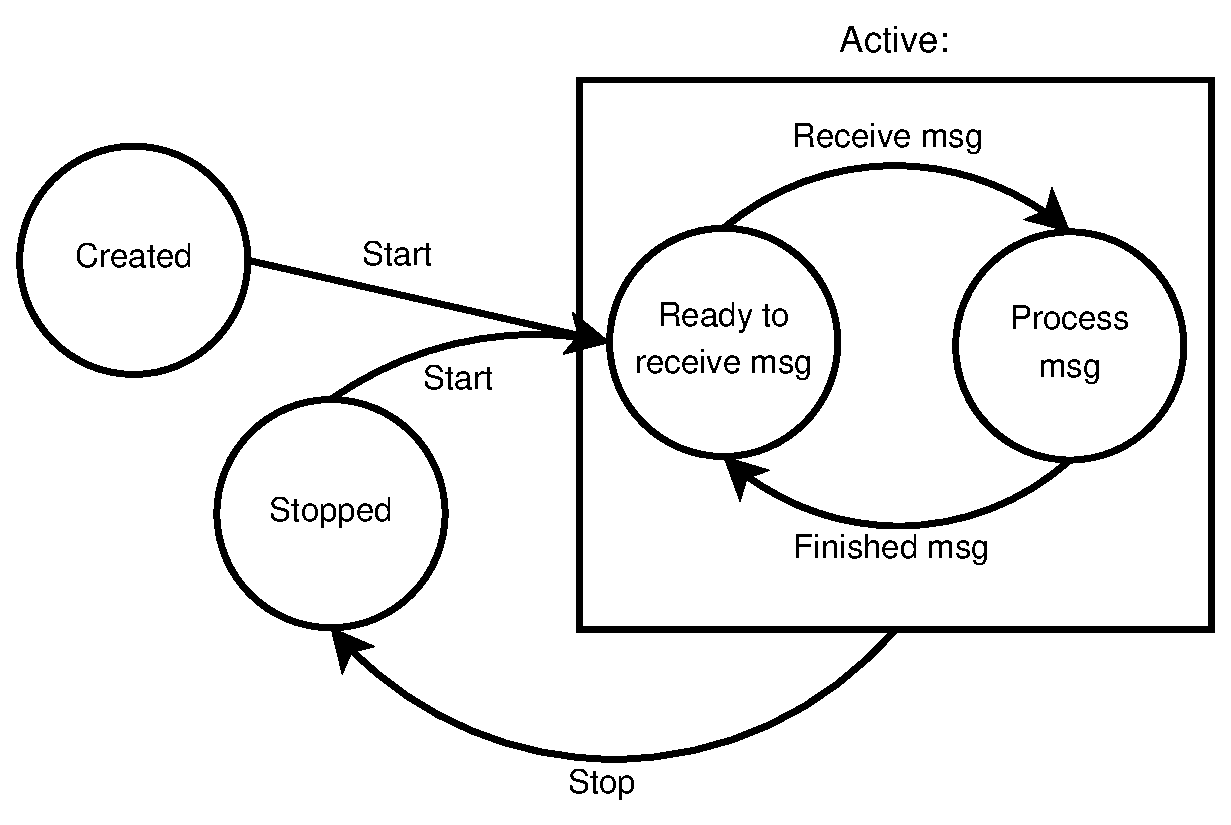
\includegraphics[scale=0.5]{\rootpath/worksheets/actor/figures/actor_lifecycle}
\caption{Lifecycle of an actor inspired by \cite[Figure 12]{subramaniam2011programming}}\label{fig:actor_lifecycle}
\end{figure}
\subsection{Modify Internal State or Behaviour}
In the last case an actor can choose to modify internal state or behaviour. Each actor has internal isolated state where only the actor itself is responsible for and allowed to modify its state. Furthermore actors have internal behaviour, typically in the form of behaviour methods, which describes how a certain type of message should be handled. For example if an actor receives an \bscode{A} message it will use the \bscode{A} behaviour method, similarly  if an actor receives a \bscode{B} message it will use the \bscode{B} behaviour method. When an actor modifies internal behaviour it will take effect for the next message to be processed. So in the third case an actor can modify internal state by updating state or change the internal behaviour by changing one or more behaviour methods. 

\subsection{Mailbox and Message Order}\label{ssec:mailbox_and_message_order}
A single actor may receive many messages in a short time which it must be able to handle without failing. To accommodate this, each actor has an associated mailbox where messages sent to the actor are buffered\cite[Chap. 2.6]{haller2012actors}. Messages can arrive in the mailbox at any time and it will hold the messages until the actor has processed them. An actor will retrieve one message at a time from its mailbox and process it in one atomic step\cite[p. 2]{karmani2009actor}.

The arrival order of messages to an actor is non-deterministic due to the asynchronous message passing communication between actors\cite[p. 2]{karmani2011actors}. Messages may take arbitrary long time to arrive because of arbitrary communication delays on the network. The actor model assumes a notion of fairness which means that messages sent are eventually received by the target actor and no actor is starved\cite[Chap. 2.5]{haller2012actors}\cite[p. 3]{karmani2009actor}. This makes reasoning about actor programs easier\cite{tasharofi2013scala}. However, in a real system there are many reasons why a message can be lost, e.g. a computer may crash resulting in lost messages which means the target actor will never receive these messages. It is up to the individual actor framework to adhere to the actor models principle of reliable message passing, often accomplished through redundancy and replication\cite[Chap. 2.5]{haller2012actors}. Another reason that message arrival is non-deterministic is that there can be many concurrently running actors which may send messages in between two messages from an actor as in the following example:
\begin{verbatim}
B ! "hello"
B ! "there"
\end{verbatim}
Suppose an actor \bscode{A} sends the two messages ``hello'' and ``there'' to an actor \bscode{B}. Another concurrently running actor \bscode{C} may then send a message in-between the ``hello'' and ``there'' messages to actor \bscode{B} thereby changing the message order. We will talk about the implications of a non-deterministic message order later in \bsref{ssec:nondeter_msg_order}.

\subsection{Example of an Actor system}
An actor system consists of a collection of actors. \bsref{fig:actor_overview} presents an illustration of the life cycle within an actor system. Each actor has an associated mailbox, isolated state and a number of behaviour methods. Actor \bscode{A} starts by sending a message to actor \bscode{B}, stored in the mailbox associated to actor \bscode{B}. Then at some point when actor \bscode{B} is ready it retrieves the message send by actor \bscode{A} from his mailbox and processes it based on which behaviour method the message corresponds to. In this case it corresponds to a behaviour method which creates a new actor, namely actor \bscode{C}. Actor \bscode{C} is now live and running with the other two actors awaiting messages. This is just a small view of what may happen in an actor system, meanwhile there may be other different actors concurrently running, sending messages, modifying isolated state and processing.

\begin{figure}[h!]
\centering
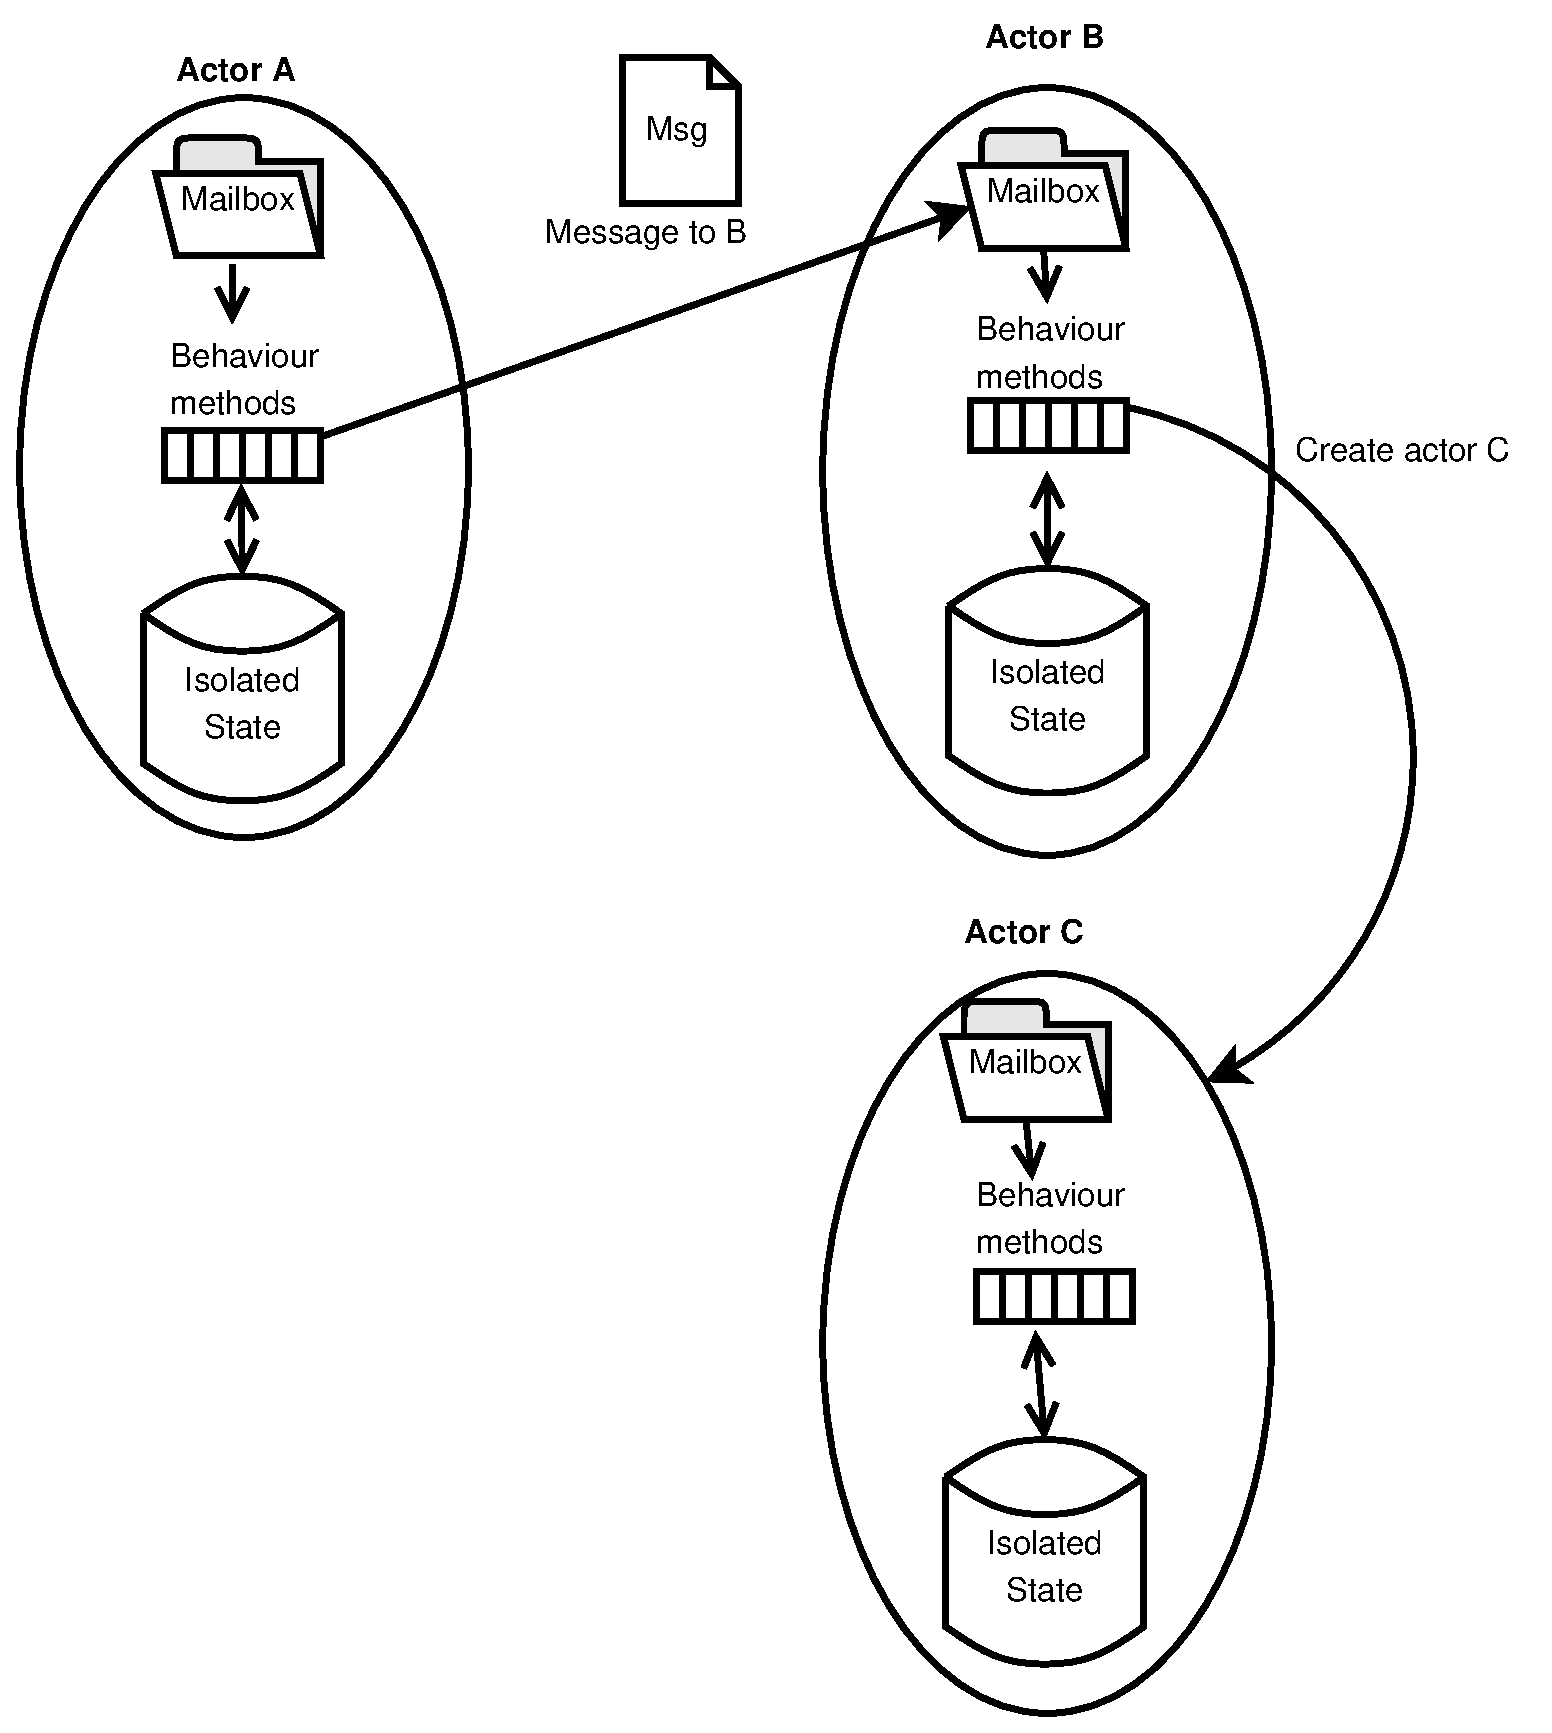
\includegraphics[scale=0.5]{\rootpath/worksheets/actor/figures/actor_diagram_overview}
\caption{Example of three actors. Each actor has its own mailbox, isolated state and methods. Actors responds to messages based on internal behaviour. Actor A sends Actor B a message which then creates Actor C.}\label{fig:actor_overview}
\end{figure}

\subsection{Semantic Properties}\label{ssec:actor_s_properties}
The actor model has several important semantic properties some of which we have already covered, namely atomic processing of messages and fairness, additionally we will now look further at encapsulation and location transparency which we have only briefly described until now\cite{karmani2011actors}.

\subsubsection{Encapsulation}
Each actor must be isolated from one another, only communicating through asynchronous message passing. An actor can therefore only modify the state and behaviour methods belonging to itself. Furthermore message passing must adhere to the principle of encapsulation by not sharing state between actors, so message passing should have call by value semantics, often done by making a deep copy of the message contents\cite[p. 2]{karmani2009actor}. Encapsulation makes it easier to reason about programs modelled with the actor model\cite[p. 3]{karmani2009actor} and reduces concurrency issues which we look at in \bsref{sec:actor_con_issues}. Another benefit of encapsulation is that it eases testing of actor programs because actors can be tested in isolation. However it is on the premise that the tests must use the same types of messages and expected message order as the live environment\cite[p. 151]{sevenModels}.

\subsubsection{Location Transparency}
Actors know each other only by unique address, often in the form of an actor name, disjointed from the physical location. Location transparency provides an abstraction where the programmer does not have to worry about or specify the actual physical location of the message recipient. An actor can communicate with another actor which exists on the same core, on the same machine or on an entirely different machine across the network\cite[p. 3]{karmani2009actor}. Location transparency gives the ability at runtime to distribute execution across a cluster of machines which eases scaling beyond a single machine.

\section{Concurrency issues}\label{sec:actor_con_issues}
In this section we present how the actor model relates to the relevant concurrency issues presented in \bsref{sec:tl_ci}.\toby{Har vi også raceconditions med her hvor jeg referer til?}
%priority inversion er ikke taget med fordi den ikke er gælende i actors
%livelock er ikke med, fordi vi (mener) at den ikke er gældende

\subsection{Race conditions}
One of the main differences from other concurrency models, such as \ac{TL} and \ac{STM}, is that there is no notion of shared state in the actor model. Instead each actor has isolated state where only the actor itself is responsible and allowed to modify state. An actor can only affect the state of another actor indirectly by message passing and the receiving actor is then responsible for changing the state. The reason that message passing as the only communication and isolated state is preferable over shared state is that race conditions are avoided by design. To exemplify this imagine two messages sent to an actor that wants to read and modify a state variable of the actor. The actor processes each message in one isolated atomic operation which means that the messages will not interfere with one another, as the messages will be processed one at a time.
%subsec:race_coditions

\subsection{Deadlocks}\label{ssec:actor_deadlock}
The concurrency issue of deadlocks is still a problem in the actor model. The actor model limits the communication to asynchronous message passing only. This helps avoid blocking waits which thereby helps to keep the program free of deadlocks\cite[p. 304]{tasharofi2013scala}. However, asynchronous message passing introduces non-determinism which in some cases is undesirable e.g. an actor buying stocks would like to know the stock quote from an actor broker before deciding whether to buy a stock or not. We will discuss non-deterministic message order further in \bsref{ssec:nondeter_msg_order}. One way to prune this non-determinism is by implementing actors by busy-waiting for the response from another actor. An example of such a busy-waiting actor program is shown in \bsref{lst:actor_busywait}. On line 5 there is an isolated integer state variable for the \bscode{BusyActor} while the behaviour methods are defined on lines 7-20. There are three different behaviour methods for the Start, Wait and Value messages. The \bscode{BusyActor} desires to busy-wait for the \bscode{OtherActor} which it does by sending 

The \bscode{BusyActor} starts by sending a message to the \bscode{OtherActor} and starts the busy-waiting by sending the \bscode{Wait} message to itself. The behaviour method for \bscode{Wait} on line 11-17 shows that the actor will print the result if it has received the result from the \bscode{OtherActor}, otherwise it will again send itself a \bscode{Wait} message. This behaviour continues until the \bscode{BusyActor} receives the \bscode{Value} message from the \bscode{OtherActor}. 

\begin{lstlisting}[label=lst:actor_busywait,
  caption={Busy-waiting actor program written in the Scala Akka actor framework.},
  language=Java,  
  showspaces=false,
  showtabs=false,
  breaklines=true,
  showstringspaces=false,
  breakatwhitespace=true,
  commentstyle=\color{greencomments},
  keywordstyle=\color{bluekeywords},
  stringstyle=\color{redstrings}]  % Start your code-block
	
	import akka.actor._
	
	class BusyActor extends Actor {
		//State
		var result : int  = 0;
		//Behaviour methods
		def receive = {
			case Start =>
				OtherActor ! Calc
				self ! Wait
			case Wait =>
				if(result > 0){
					println(result)
				}
				else{
					self ! Wait
				}	
			case Value(i: int) =>
				result = i
		}
	}
\end{lstlisting}
It is possible to obtain a deadlock by two or more actors awaiting messages from one another. An illustration of a deadlock between two actors is shown \bsref{fig:actor_deadlock}.

\begin{figure}[ht!]
\centering
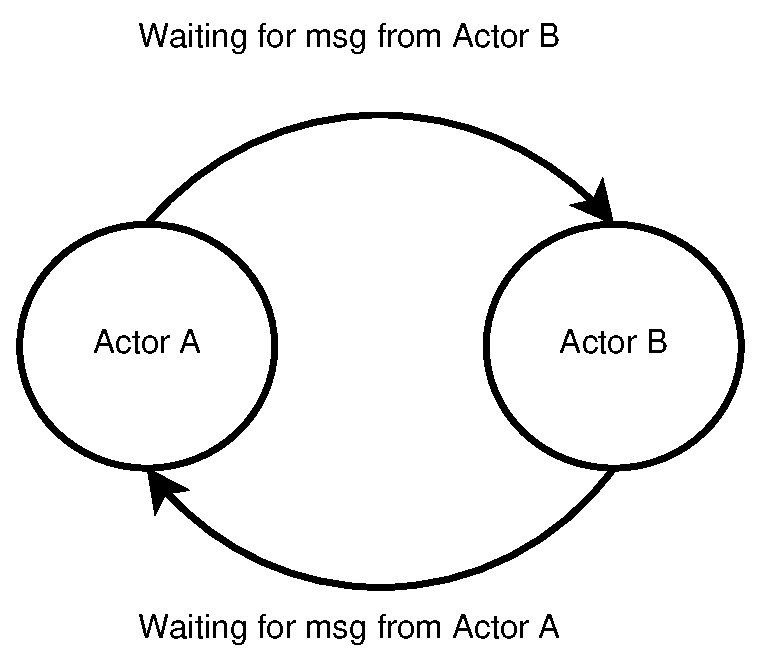
\includegraphics[scale=0.5]{\rootpath/worksheets/actor/figures/actor_deadlock}
\caption{Example of a deadlock between two Actors}\label{fig:actor_deadlock}
\end{figure}

A deadlock with busy-waiting actors does however still enable other actors, unrelated to the deadlock, to send and receive messages from a deadlocked actor. This is illustrated on \bsref{fig:actor_deadlock_otheractor} where \bscode{Actor C} sends an \bscode{Other} message in-between \bscode{Actor A's} infinite busy-waiting messages. This means that even when a deadlock occurs the rest of the actor system, unrelated to the deadlock, will still be able to run.

\begin{figure}[ht!]
\centering
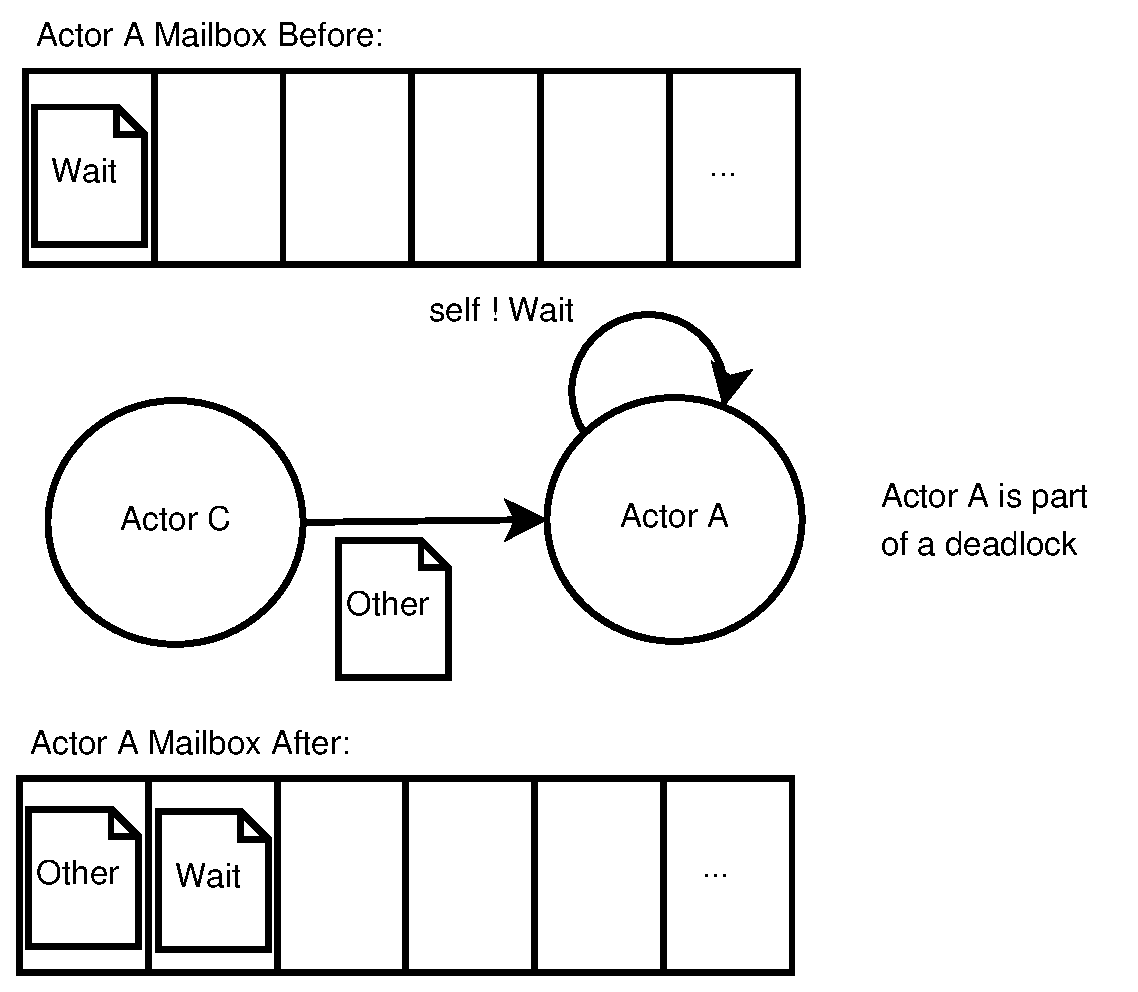
\includegraphics[scale=0.5]{\rootpath/worksheets/actor/figures/actor_deadlock_otheractor}
\caption{Example of an actor C, unrelated to the deadlock, that sends a message to a deadlocked actor A. The message will will be retrived and reacted on by Actor A.}\label{fig:actor_deadlock_otheractor}
\end{figure}

%not as fatal as a deadlock in TL?
\subsection{Starvartion}
The fairness semantic property of the actor model, presented in \bsref{sec:actor_concepts}, assumes that a message sent is eventually received by the target actor and that no actor is permanently starved. This means that in the actor model there is no starvation concurrency issues. However in some actor implementations starvation is present, one reason is that it may not be possible to adhere to the fairness property in an actor framework for an existing language. We will discuss more about adhering to actor properties in \bsref{ssec:adhere_actor_prop}.
%Evt. referer til busy-wait eksmeplet og forklar hvordan det er muligt at have starvation deri
\section{Discussion}\label{sec:actor_discussion}
This section discusses a number of issues and weaknesses related to the actor model. Behaviour sharing in the actor model is discussed in \bsref{ssec:share_behaviour}, followed by a discussion of actor modelling in \bsref{ssec:actor_modelling}. Hereafter we look at the non-deterministic message order present in the actor model in \bsref{ssec:nondeter_msg_order}. The last two sections are more actor implementation oriented where we first in \bsref{ssec:abstraction_over_threads} describe the relation between actors and threads and lastly in \bsref{ssec:adhere_actor_prop} discuss adherence to actor properties in actor implementations.\toby{Hvis der kommer flere sektioner, indsæt her.}

\subsection{Sharing Behaviour Among Actors}\label{ssec:share_behaviour}
Inheritance is a popular and valuable mechanism often used in object-oriented programming which allows sharing of the same behaviour inside one class across multiple classes\cite{kafura1989inheritance}. So if two classes have some common functionality, it can be written only once in a super class that they both inherit from. Sharing of behaviour avoids code duplication and code reuse which also improves maintainability as the functionality should only be maintained in a single place.

In the actor model there is no direct notion of inheritance\cite{mackay1997has}. This means that it is not possible to share behaviour among actors which hurts code reuse, maintainability and makes it more time consuming to write actor programs with common behaviour. The problem of inheritance in the actor model is that actors may change behaviour over time so it is difficult to locate or copy methods at run-time in systems without shared memory\cite{kafura1989inheritance}.\toby{kig på evt. på "inheritance in actor based concurrency object-oriented lanuages" de mener der er et mere fundamentalt problem, se afsnit "4. the actor-inheritane problem" - jeg forstår det dog ikke helt - måske en anden skal se om de kan forstå det. (de har også en mulig løsning - som dog har en limitation)}

In some specific implementations of the actor model it is possible to use inheritance in combination with actors e.g. \cite{kafura1989inheritance} presents a possible solution in their ACT++ language. However in ACT++ they do not adhere to the fundamental principle of the actor model that an actor can change behaviour over time. 

An indirect way to share behaviour among actors is to use the features of the language an actor framework is implemented in e.g. in an actor framework for Scala it is possible to use the object-oriented features such as traits to share behaviour among actors.\toby{Ved ikke om jeg bare skal lade være med at nævne dette. Jeg tænker på eksempler fra dette link: http://stackoverflow.com/questions/17383827/how-do-i-best-share-behavior-among-akka-actors}
%Måske brug den her også
%Kilde også om inheritance \cite[Chap. 1.2]{agha1986overview}

\subsection{Actor modelling}\label{ssec:actor_modelling}
One of the main properties of the actor model is that an actor processes only a single message at at time. This means that no matter what type of messages that are in the mailbox, they are processed sequentially, which can result in a lower degree of concurrency for several messages only interested in ``reading'' the internal state of an actor. Messages should be fairly coarse-grained so actors can process sufficiently many tasks concurrently without having to spend time waiting for each other\cite[p. 269]{karmani2009actor}. Furthermore as the communication is through message passing it is more attractive to have coarse-grained messages to avoid unnecessary overhead by sending a lot of small messages. However messages should not be too coarse-grained as that will hurt the dynamics among actors in the system e.g. if an actor \bscode{A} is processing a very time consuming message and another actor \bscode{B} needs a simple read of actor \bscode{A's} isolated state to continue, actor \bscode{B} must await until actor \bscode{A} is finished processing.
%Extra (the essence of it is described above i think)
	%because actors do not share state and can only communicate through message passing, they are not a suitable choice if you need fine-grained parallelism. (seven models)
	%not all applications are well-suited for an actor-based model. Actors serve well when we can divide the problem into parts that can run quite independently and need to communicate only sporadically. If frequent interaction is required or the parts or tasks need to coordinate to form a quorum, the actor-based model is not suitable. We may have to mix other concurrency models or consider significant redesign. (jvm mastering bogen)

\subsection{Non-deterministic message order}\label{ssec:nondeter_msg_order}
The asynchronous message passing is a key source to the non-determinism present in the actor model, as earlier mentioned in \bsref{ssec:mailbox_and_message_order}. That the message order is non-deterministic means that an actor must not rely on a specific message order, however according to \cite[p. 35]{haller2012actors}: \textit{``You can often alleviate reliance on message ordering by refactoring the actor communication, i.e., reworking the messages' contents''}. In some cases that does not suffice and the programmer must prune some of the non-determinism by restricting the order in which messages are processed. For example an actor \bscode{A} requests a stock quote from a broker actor \bscode{B}, then actor \bscode{A} must await the response of actor \bscode{B} to be able to decide whether to buy the stock or not. An illustration of the example is illustrated in \bsref{fig:request_reply_pattern}. The scenario described uses the request-reply pattern which is one of the most common patterns of messaging and synchronization in actor programs\cite[p. 5]{karmani2009actor}.

\begin{figure}[h!]
\centering
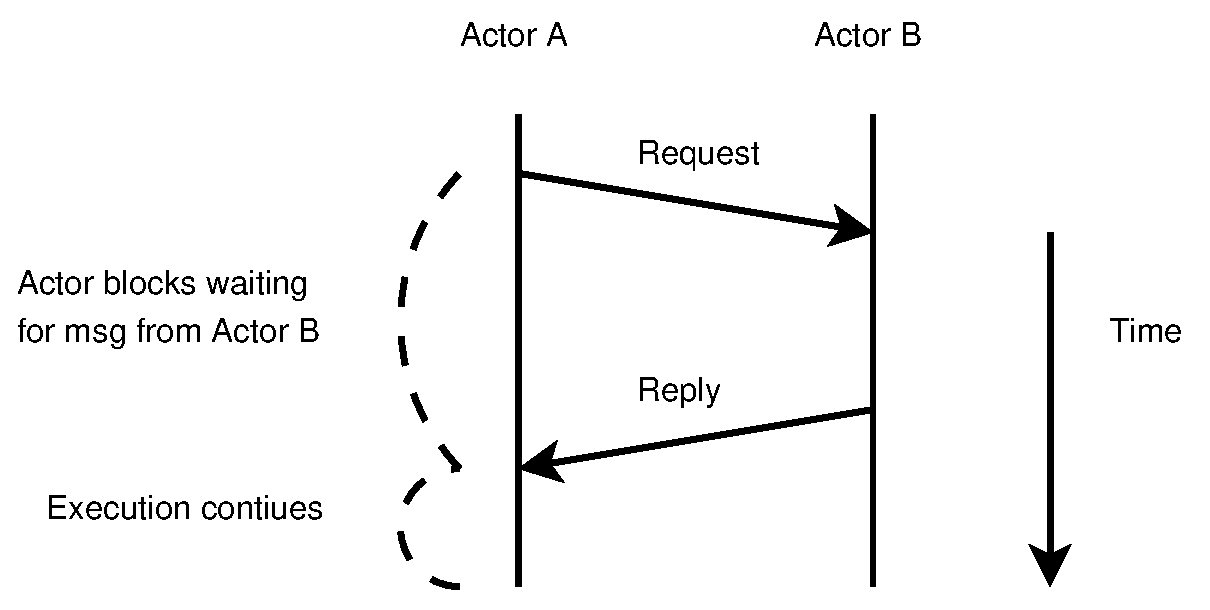
\includegraphics[scale=0.6]{\rootpath/worksheets/actor/figures/request_reply_pattern}
\caption{Request-reply pattern where actor \bscode{A} blocks until it recevies the response from actor \bscode{B}. Other messages received while blocking is saved for later processing.}\label{fig:request_reply_pattern}
\end{figure}

To implement the request-reply pattern the programmer has to explicitly program the following steps: an actor send request, wait for reply to arrive and for each incoming message check if it is a reply to the request or another message. If the request-reply pattern is used numerous times within one program it will quickly result in unnecessary code duplication which is why the pattern is almost universally supported as a programming abstraction in actor implementations\cite[p. 5]{karmani2009actor}.

There exists a number of other different programming abstractions for communication and synchronization in actor programs which differ depending on the choice of actor implementation\cite[p. 6]{karmani2009actor}. An alternative to request-reply is local synchronization constraints which enables the programmer to postpone the processing of a message until it receives some sequence of messages or until a condition on the actors state is met.

However pruning the non-deterministic nature of asynchronous message passing in the actor model is not without implications. If the communication is restricted to blocking and synchronous operations it can lead to deadlocks, as we saw an example of with two busy-waiting actors in \bsref{ssec:actor_deadlock}. The limitation to asynchronous message passing helps avoid deadlocks but it adds to the complexity of coordination\cite[p. 311]{tasharofi2013scala}.

\subsection{Abstraction Over Threads}\label{ssec:abstraction_over_threads}\toby{Maybe also something about at some level lock acquire/release is required and it is not free - Bent's slides (coordinating message queues, locking is still required)}
The actor model provides simple constructs such as actors, mailboxes and messages to construct concurrent programs. However, these constructs are used as an abstraction that builds on top of the conventional threads and it is the responsibility of the individual actor implementation to map actors to threads. A naive solution is to map each actor onto a single thread but an actor system may consist of a large number of actors, resulting in a large overhead for thread creation and context switching\cite[p. 7]{karmani2009actor}. A more efficient solution is to have a light-weight actor to thread mapping where each actor is not directly mapped to a thread. This can be accomplished by having a fixed thread pool and using continuation based actors where the actor and its state is encapsulated in a continuation. The threads in the thread pool all share a common scheduler queue of actors. Each thread dequeues an actor from the queue and calls its continuation. The thread will continue to run the actor until some condition is met e.g. there are no more messages in the actors mailbox. Light-weight actors reduce the number of threads which thereby reduces the overhead of thread creation, also context switch overhead is reduced by using continuations. However if the scheduling of actors is not fair it can cause starvation in the system\cite{karmani2009actor}. It is the responsibility of the individual actor implementation to ensure the semantic property of fairness and thereby avoid starvation. This leads us to the next section about adherence to actor properties in actor implementations.
%light-weight actor implemetation examples: Erlang, Akka

\subsection{Adhering to Actor Properties}\label{ssec:adhere_actor_prop}
As mentioned in \bsnameref{sec:prelim} there exist several actor implementations both directly as actor languages and indirectly through actor frameworks for existing languages. As the actor model is a conceptual model, it is up to the individual actor implementation to adhere to the semantic properties of the actor model, mentioned in \bsref{ssec:actor_s_properties}. Some actor implementations choose not to adhere to one or more of the actor properties as they introduce a performance overhead. In \cite{karmani2009actor} they present a comparison of actor frameworks on the JVM platform where only half of the compared frameworks support all of the semantic properties of the actor model. 

\subsubsection{Safe Message Passing}
The only form of communication in the actor model is message passing. A disadvantage of message passing is that it may produce a high communication overhead, because processes need to create and send messages, and these must be buffered in the mailbox before they can be received to support asynchronous message passing\cite[p. 17]{haller2012actors}. Furthermore, safe messaging requires call by value semantics which often involves deep copying message contents, which is an expensive operation for large messages. To reduce the overhead of message passing, some actor implementations chooses to implement message passing by sending message contents by reference opposed to deep copying message contents.\toby{Skal vi have eksempler på nogle der gør det? Akka og Kilim gør det f.eks.} However, this reintroduces the concurrency issue of race conditions, as multiple actors can have access to the same shared memory directly through the reference. For example one actor may use the reference inside a message to change the state of another actor directly, opposed to only being able to do it indirectly through a message as the conceptual actor model states. The actor implementations that send message contents by reference put the responsibility of ensuring safe messaging on the programmers, which can be done e.g. by using immutable messages or less strictly, simply not changing any message contents. It is often a trade-off between performance and adhering to all the semantic properties of the actor model, in that you loose some of the advantages of using the actor model by getting a performance gain.\toby{Måske også snak om det i forhold til et distriburet mlijø (der har vi ikke dele state, så her er det ikke så gældende - medmindre man forsøger at sætte actor der snakker meget sammen, på samme node)}
%another way for developers to manually handle it is to deep copy message contents which may be modified and refernece others (for example large messages)
%Akka can’t enforce message immutability (yet) so this has to be by convention. (http://doc.akka.io/docs/akka/snapshot/java/untyped-actors.html)

\subsubsection{Unbounded Mailbox}
In the conceptual actor model the mailbox is unbounded, meaning that it is possible to store infinitely many messages in an actors mailbox. However, in an actual actor implementation there exists an upper limit on how many messages that can be stored based on how much physical storage is available. The consequence of an upper limit of messages in a mailbox is that it makes it possible to overflow the mailbox which can cause the system to crash\cite[p. 152]{sevenModels}.

\subsubsection{Actor Framework Limitations}
An actor framework for an existing language is more limited than an actor based language, as doing program transformations, compilation and runtime optimizations to gain better performance is less challenging\cite[p. 5]{karmani2011actors}.\toby{Ændr sætning og hav fokus på at det er fordi at man har muligheder for at lave optimeringer i sin kompiler til at gøre det lettere. Og man er ikke restirced af det exsisting langague} Another disadvantage of an actor framework in an existing language is that you are writing normal code from the existing language within you actors, which may not constrain the programming environment sufficiently to support the actor model. An example of this can be seen in \bsref{lst:actor_state_encapsulation_violation} which shows how it is possible in the Scala Actors framework to break the encapsulation property of the actor model. On line 3-12 the \bscode{CountActor} actor is defined which has a behaviour method for when it receives an \bscode{enter} message which will increment the state variable \bscode{num} if \bscode{MAX} has not been reached. On line 14-19 a main function is defined which creates \bscode{myCount} and starts it. On line 17 an \bscode{enter} message is sent to \bscode{myCount} but on line 18 behaviour method for \bscode{enter} is called directly because the \bscode{Actor} is simply a class, so it is possible to call the methods within a class in Scala. The encapsulation property of the actor model is broken because an actor must only be able to execute the behaviour method of another actor indirectly through a message and not directly. In this case it may cause two actors to simultaneously execute the \bscode{enter} method which can lead to race conditions. 

\begin{lstlisting}[label=lst:actor_state_encapsulation_violation,
  caption={Scala Actors violating state encapsulation},
  language=Java,  
  showspaces=false,
  showtabs=false,
  breaklines=true,
  showstringspaces=false,
  breakatwhitespace=true,
  commentstyle=\color{greencomments},
  keywordstyle=\color{bluekeywords},
  stringstyle=\color{redstrings}]  % Start your code-block
	
	import scala.Actors.Actor
	
	class CountActor() extends Actor {
				
		...
		
		def enter(){
			if(num < MAX){
				num = num + 1;
			}
		}
	}
	
	def main(args : Array[String]) : Unit = {
		var myCount = new CountActor();
		myCount.start
		myCount ! "enter"
		myCount.enter
	}
\end{lstlisting}

The programmer may therefore have to be observant not to violate the semantic properties of the actor model by mistake, when using an actor framework for an existing language.

%evt. til slut i sektionen referer til jvm comparision og de kommer frem til at man godt kan have et jvm framework der understøtter alle actor properties og samitdig har "comparable" performance med andre actor frameworks der ikke gør det.

%Unfortunately, actor frameworks on the JVM cannot sufficiently constrain the programming environment to avoid the concurrency pitfalls that the actor model should help you avoid. After all, within the thread you are simply writing plain old java (or scala or clojure). There’s no real way to limit what that code can do, unless it is explicitly disallowed from calling into other code or looping. Therefore, even the actor frameworks which use bytecode weaving to implement cooperative multi-tasking amongst actors cannot fully guarantee non-blocking behavior. This point bears repetition: without fundamental changes in how the JVM works, one cannot guarantee that an arbitrary piece of code will not block. fra: http://boundary.com/blog/2014/09/03/no-you-cant-have-a-pony/

\toby[inline]{Evt. også afsnit om at actor modellen blandes med andre concurrency modeller (tag udgangspunkt i den artikel i dropperen)}
%Noget fra artiklen om at man tit anvender andre concurrency værktøjer, end kun actors artikeln (sammen med actors).
	%bl.a. actor model og libray inadequecies og evt. også konklussionen

%EKSTRA:
	%the argument for using actor-based programming languages is not simply that they are a good match for distributed computing platforms; it is that Actors is a goodmodel in which to think about concurrency. Actors simplify the task of programming by extending object-based design to concurrent (parallel, distributed, mobile) systems (nye blue hand book lige før biblografi)
\section{Actor Characteristics}\label{sec:actor_charac}
This section presents how the actor model relates to the selected characteristics presented in \bsref{chap:char}.\toby{Overskrift kunne være: actor model char evaluation?}

\subsection{Implicit or Explicit Concurrency}
The actor model hides the low level concepts of threads and locking. While it builds upon them, they are implicitly handled by the actor system. The actor model does however expose a number of new constructs in the form of creating actors, sending message and modifying isolated state or behaviour which must be explicitly handled by the programmer. Concurrency is introduced by creating actors and communicating is done explicitly by sending messages. As such we say that the actor model is a explicit concurrency model. This is shown in BLA\toby{indsæt ref}.

%The actor model specifics concurrency and synchronization implicitly as a result of having only isolated mutable state and atomic processing of messages. The mailbox and atomic processing serves as an implicit synchronization point which ensures only a single entity will access mutable state at a time. A consequence of this design is that all state variables in an actor program are implicitly ensured mutual exclusion, unlike in \ac{TL} where you explicitly have to choose which state variables to cover. BLA\toby{indsæt ref} shows that the actor model is very implicit.\toby{Begrund hvorfor, hvis vi ikke sætter den helt til venstre}

\missingfigure{Figur der viser actor er implicit (langt til venstre, og evt. længere end STM)}

\begin{figure}[htbp]
\centering
 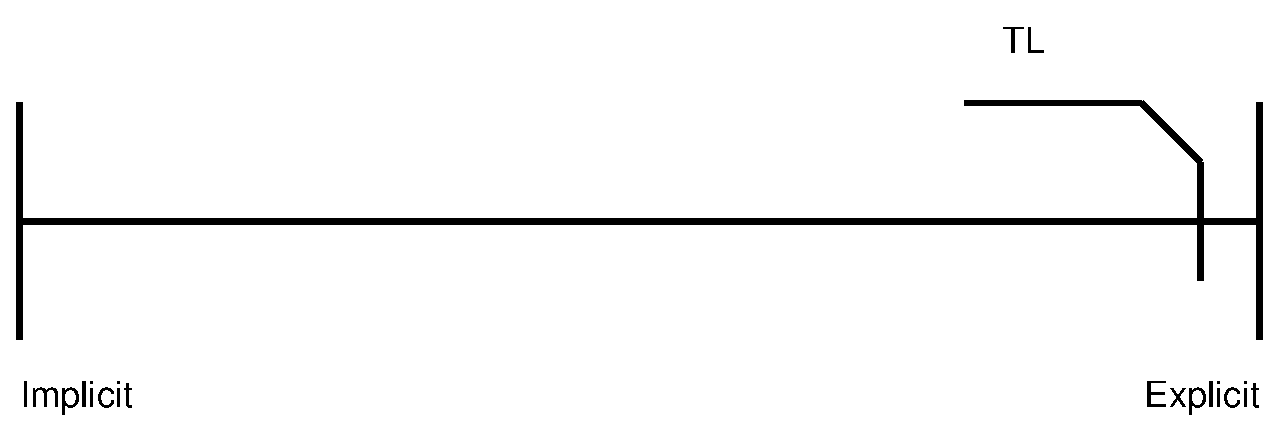
\includegraphics[width=0.9\textwidth]{\rootpath/worksheets/actor/figures/characteristics/actor_char_implicit_explicit} 
 \caption{The actor model on the Implicit - Explicit concurrency spectrum}
\label{fig:actor_implicit_explicit}
\end{figure}
\subsection{Fault Restrictive or Expressive Model}\label{sec_actor_fault_express}
The actor model forces some limitations on the programmer. The biggest limitation is that the model prohibits the use of shared mutable state and only allows isolated mutable state. Another limitation is that communication is limited to asynchronous message passing between actors solely. Furthermore, the atomic processing of messages ensures that only a single entity accesses mutable state at a time, however this disallows multiple read operations to happen simultaneously which is reasonable in regards to mutual exclusion. The actor model only permits the programmer to model the program by modelling individual actors and how they interact with one another. Based on these observation we say that the actor model is fault restrictive as shown in BLA\toby{indsæt ref}.\toby{Forklar hvorfor vi præcist sætter den hvor vi gør}

\missingfigure{Figur der vist actor er faul restictive (ved ikke hvor langt til venstre helt, men nok længere end STM)}
\begin{figure}[htbp]
\centering
 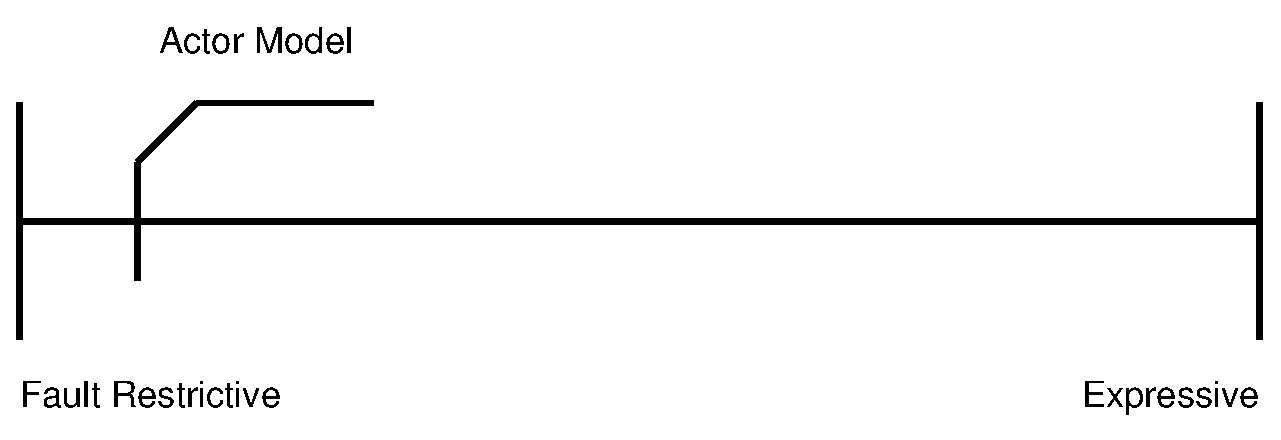
\includegraphics[width=0.9\textwidth]{\rootpath/worksheets/actor/figures/characteristics/actor_char_fault_expressive} 
 \caption{The actor model on the Fault Restrictive - Expressive spectrum}
\label{fig:actor_fault_expressive}
\end{figure}

\subsection{Pessimistic or Optimistic Model}
The atomic processing of messages facilitates a pessimistic approach, as it allows only a single message to be processed at a time which ensures only a single entity will access some mutable state at a time. Race condition issues are therefore avoided by design and a recovery mechanism for two entities simultaneously doing conflicting operations on mutable state is not needed. The actor model is in fact very pessimistic, as it enforces upon all state variables that only a single entity may access it at any given time. This can introduce unnecessary wait overhead if there are many immutable variables, that could have been accessed simultaneously safely. However, if the semantic property of state encapsulation is not adhered to in an actual actor implementation, it is possible to access the isolated state of another actor directly without sending a message, as illustrated earlier in \bsref{lst:actor_state_encapsulation_violation}. An important thing to note is that breaking state encapsulation introduces race conditions again, which the conceptual actor model carefully avoids by design, so there is no recovery mechanism for it.\toby{Evt. slet de to sætninger om ikke at adhere til det, eller hvad synes i?} On BLA\toby{indsæt ref} the placement visualizes the degree of how implicit the actor model is.\toby{Forklar hvorfor den netop står hvor den gør}

\missingfigure{Meget pessimistic evt. mere pessimistisk end TL, fordi den restrictier access for alle state varaibler automatisk, hvor man i TL skal vælge hvilke hvilke variabler man gør det på. Det betyder at man kan unlade at gøre det på nogle, f.eks. de der ikke er mutable, men final immutable variable (det kan man ikke i actor).}
\begin{figure}[htbp]
\centering
 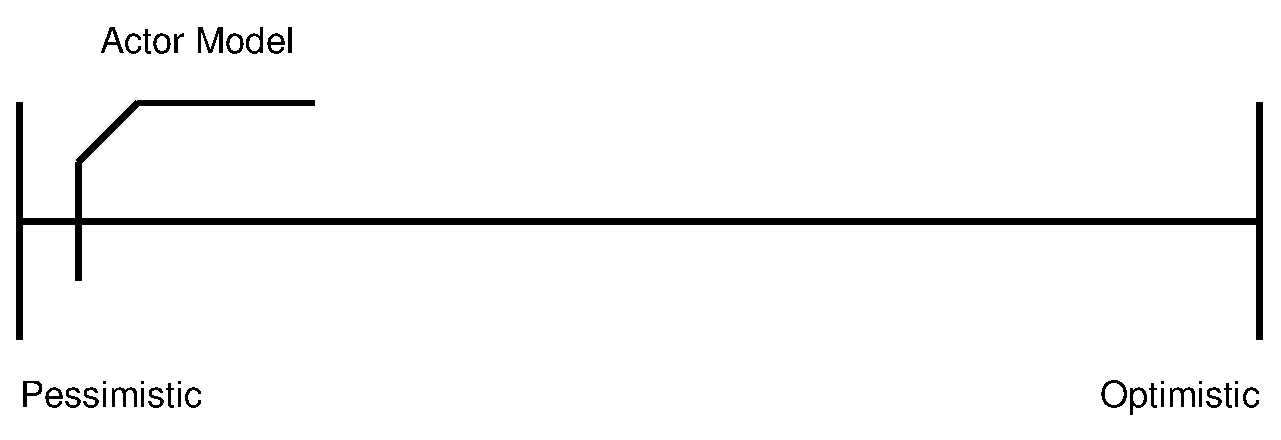
\includegraphics[width=0.9\textwidth]{\rootpath/worksheets/actor/figures/characteristics/actor_char_pessimistic_optemistic} 
 \caption{The actor model on the Pessimistic - Optimistic spectrum}
\label{fig:actor_pes_opti}
\end{figure}

\subsection{Readability \& Writability}
We will base the evaluation of readability \& writability upon the same procedure as in \bsref{subsec:tl_charac_read_and_write}, due to the same concerns. First, the sub characteristics simplicity and orthogonality are evaluated for both readability \& writability, followed by an evaluation of the readability of the actor model. Afterwards the remaining sub characteristics for writability, level of abstraction and expressivity, is evaluated. Finally an evaluation of the writability of the actor model is presented.

\subsubsection{Simplicity}\label{subsec:actor_simplicity_read}
The actor model provides a fairly simple concurrency model, as race conditions are avoided by design and also help avoiding deadlocks, if the semantic properties are adhered to and the non-deterministic nature of asynchronous message passing is embraced, as discussed in \bsref{ssec:nondeter_msg_order}. However the actor model has a number of issues discussed in \bsref{sec:actor_discussion} that contributes negatively to its simplicity.\toby{Skal jeg uddybe mere på det gode, eller passer dette fint?}

The actor model requires a different mindset than programmers are used to in the imperative and \ac{OOP} paradigms where they promote shared mutable state. The actor model relies solely on isolated mutable state. Inadequate programmer experience can impact the simplicity of the actor model negatively initially, until programmers are accustomed to this new mindset.\toby{Skal vi uddybe lidt mere på det og smide det op i actor discussion? Så det ikke først kommer ind her. (det affecter vel også readability og writability. Eller skal vi have en helt ny characteristic: Cost, som indeholder programmør læringstid af modellen, maintainability og evt. mere?} Furthermore, sharing of behaviour among objects, in the form of inheritance, is common for developers to do in \ac{OOP}, but it is not possible in the actor model as discussed in \bsref{ssec:share_behaviour}. This impacts the simplicity negatively as in the case of common behaviour code duplication is necessary.\toby{Også dårligt i forhold til maintainability}

The non-deterministic message order is not suitable for every situation e.g. the stock example, as discussed in \bsref{ssec:nondeter_msg_order}. The conceptual actor model does not provide any constructs to prune away this non-determinism, so the programmer  must build patterns for coordination manually. This hurts the simplicity of the actor model as the programmer must write a lot of boilerplate code each time a certain pattern is used. However, many actor implementations provides some useful patterns for coordination, such as the request-reply pattern, which negates the negative impact on simplicity.

It is not all actor implementations that adhere to all the semantic properties of the actor model, either to obtain a more efficient implementation or because of restrictions e.g. when implementing an actor library for an existing language. If the actor implementation does not adhere to the semantic properties of the actor model, it can affect the simplicity of the actor negatively, as it puts the responsibility on the programmer to enforce the properties themselves e.g. be sure not to break state encapsulation using an actor framework for an existing language.

As discussed in \bsref{ssec:actor_modelling},  there is an overhead in creating, sending and receiving messages. So there should not be too many small messages, but also not few large messages as that will hurt the dynamics among actors. We do not find this as severe to the simplicity of the actor model as the other issues discussed, because no matter what concurrency model you use, you must be careful not to assign too much work to a single entity. \toby{Hvad siger i til det her afsnit?}\kasper{Det er bare iorden.}
%However, message size and load can be crucial to obtaining an efficient program.

The placement of the actor model on the simplicity spectrum is shown on BLA\toby{indsæt ref}. The actor model provides a fairly simple concurrency model with implicit\kasper{Skal nok ændres} concurrency that avoids race conditions by design and helps avoid deadlocks. However, there are also a number of issues discussed above which has a negative impact on the simplicity. We have therefore placed the actor model in the middle of the spectrum.\toby{Bliv enige om hvor den skal stå. Jeg er selv ikke sikker. Evt. begrund det med explicit concurrency og den abstraction man får - men stadivæk ikke nemt at lave concurrency}

\missingfigure{Længere til højre end TL, men ved ikke hvor meget?}
\begin{figure}[htbp]
\centering
 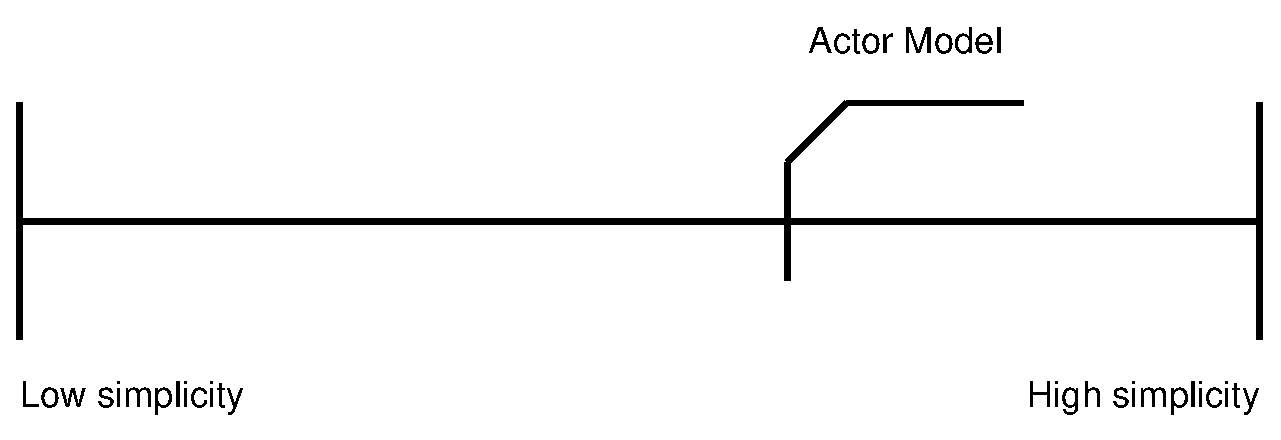
\includegraphics[width=0.9\textwidth]{\rootpath/worksheets/actor/figures/characteristics/actor_char_read_simplicity} 
 \caption{The actor model on the low - high simplicity spectrum}
\label{fig:actor_read_simplicity}
\end{figure}
%%%MORE:
%Måske noget om at man kan bruge actor modellen til at tænke over og modelere sine concurrency problmeber. (tror der står noget om det i scala actors i starten)
%the simplicity lies in that you do not have to worry about any explicit declaration as e.g. locking.
%Inadequete developer experinece, they used runnable because (kilde: scala actors mix):
	% used to traditional style of programming with shared state (Måske skriv et afsnit om det i acotr discussion)
	% legacy code they want to keep using it
	% did not want to trust a new techonology, when runnable would be enough for implementing required functionality
\subsubsection{Orthogonality}\label{sec:actor_orthogonality}
The actor model has a small amount of constructs for building concurrent programs. The main building block and abstraction is actors, that represent independent entities running concurrently. The other construct is messages, that enables communication between actors. Actors and messages can be combined in a large number of ways. An actor can however only send a message to a single actor at a time, but that can be simulated by e.g. having an \bscode{AllActor} that redirect the message to all other actors in the system. Another combination which is not directly allowed, is that only a single actor can react on a message, however that could also be simulated by modelling with additional actors. Actors can even be combined internally as an actor may create several other child actors.

Actors can be modelled and combined in a way that produces deadlocks, as discussed in \bsref{ssec:actor_deadlock}. Such combinations are not desirable and therefore not allowed if it was possible to detect such combinations. This hurts the orthogonality of the actor model as some of the combinations are not feasible. However, recall that actors in the system not part of the deadlock are not affected and can continue to run, which means violating the allowed combinations is not as fatal as in other concurrency models that stop the progress of the rest of the system.\toby{ved ikke om jeg skal ahve den sidste sætning med}

So as the actor model consists of a small amount of constructs that can be combined in a large number of ways, it seems to have a high orthogonality. However as there are some combinations that are not directly allowed and others producing deadlocks, it is not fully orthogonal. The degree of orthogonality for the actor model is shown BLA\toby{indsæt ref}.

\toby[i]{Måske noget om at man også kan deadlocke heri, hvilke restricter visse kombinationer, hvis actors modleres som blocking operationer?}

\missingfigure{orthogonal - men ikke helt oppe fordi nogle kombinationer er ikke tiladt direkte. Måske også lidt mindre i forhold til deadlocks}
\begin{figure}[htbp]
\centering
 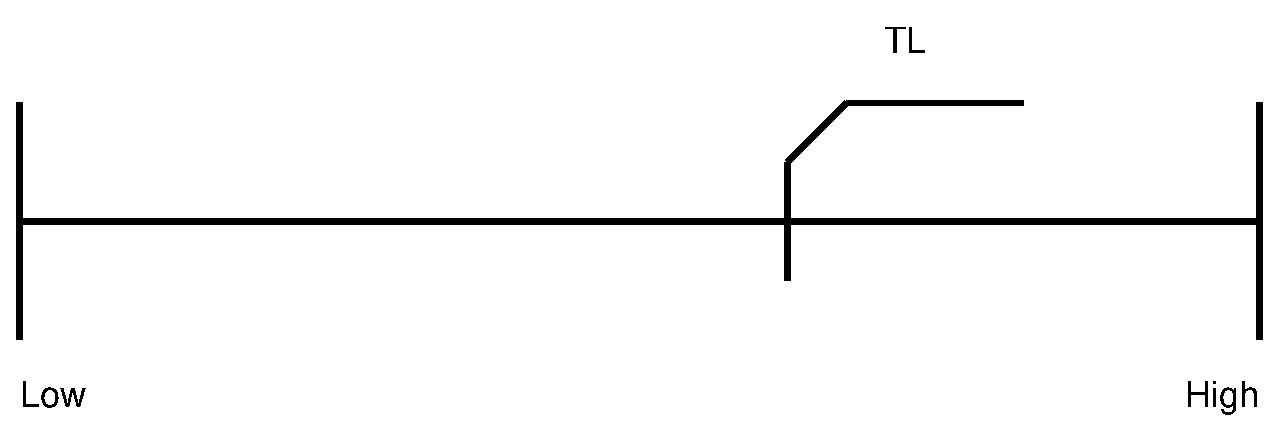
\includegraphics[width=0.9\textwidth]{\rootpath/worksheets/actor/figures/characteristics/actor_char_orthogonality} 
 \caption{The actor model on the low - high orthogonality spectrum}
\label{fig:actor_orthogonality}
\end{figure}

\subsubsection{Readability evaluation}
The simplicity and orthogonality directly influences the readability. Simplicity was placed between the middle and high end of the spectrum as it provides a fairly simple concurrency model but a different mindset is required for actor modelling and it introduces some new challenges which must be dealt with, such as non-deterministic message order. This hurts the readability of the actor model, at least until the programmer gets familiar with the different mindset and get accustomed to these challenges. Orthogonality was placed in the high end of the spectrum, as there is a low amount of constructs which is able to be combined in a large number of ways, either directly or indirectly. This influences the readability of the actor model positively.

Additionally, all code in terms of state and behaviour methods associated with an actor is encapsulated and stored within the actor, which makes it easier to understand what a given actor encompasses. A programmer reading an actor program can start out by understanding how a single actor operates and then continue to examine how the actors that it communicates with operates, eventually leading to an understanding of the entire program. However it can also have a negative impact on the readability, as the flow of the program is distributed out into the actors, so there is no single place to get an overview of the flow.\toby{Skal der snakkes mere her?} 

The readability of the actor model is shown on BLA\toby{Indsæt ref} where it is placed between middle and high readability. It is not considered to have a very high readability due to the different mindset and new challenges the model introduces, which can be hard to understand at first.

\missingfigure{Over midten? Ved ikke hvor langt til højre}
\begin{figure}[htbp]
\centering
 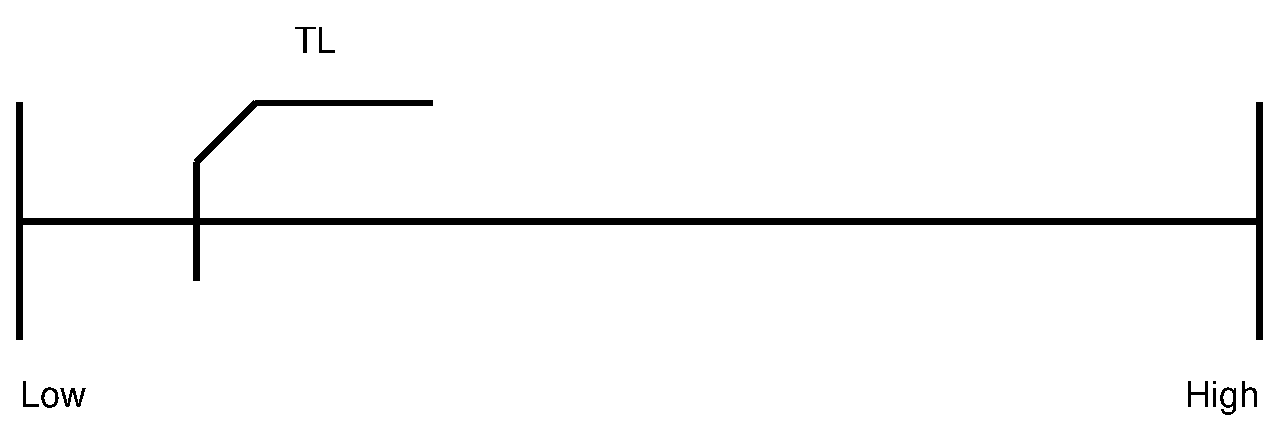
\includegraphics[width=0.9\textwidth]{\rootpath/worksheets/actor/figures/characteristics/actor_char_readability} 
 \caption{The actor model on the low - high readability spectrum}
\label{fig:actor_readability}
\end{figure}


%more: 
% you clearly see what state varaibles an actor will ensure synchronization for in the way the model dictates isolated state
\subsubsection{Level of abstraction}\label{sec:actor_level_of_abstraction}
The actor model let the programmer focus on high-level concurrency abstractions and hide the complexities that can easily lead to errors, in order to simplify concurrent programming. Synchronization is accomplished implicitly as a result of actor mailboxes and atomic processing of messages. Threads are still used under the hood to run the actors, with different implementation strategies as discussed in \bsref{ssec:abstraction_over_threads}.

These high level abstractions enables the programmer to model and think about concurrent problems conceptually in terms of actors and their interaction, without having to write the program.

Based on the above considerations we argue that the actor model has a high level of abstraction, as illustrated on BLA\toby{indsæt ref}.

\missingfigure{Høj level of abstraction. Kan vi finde noget der skader degree of level of abstraction? Synes jeg ikke jeg kan.}
\begin{figure}[htbp]
\centering
 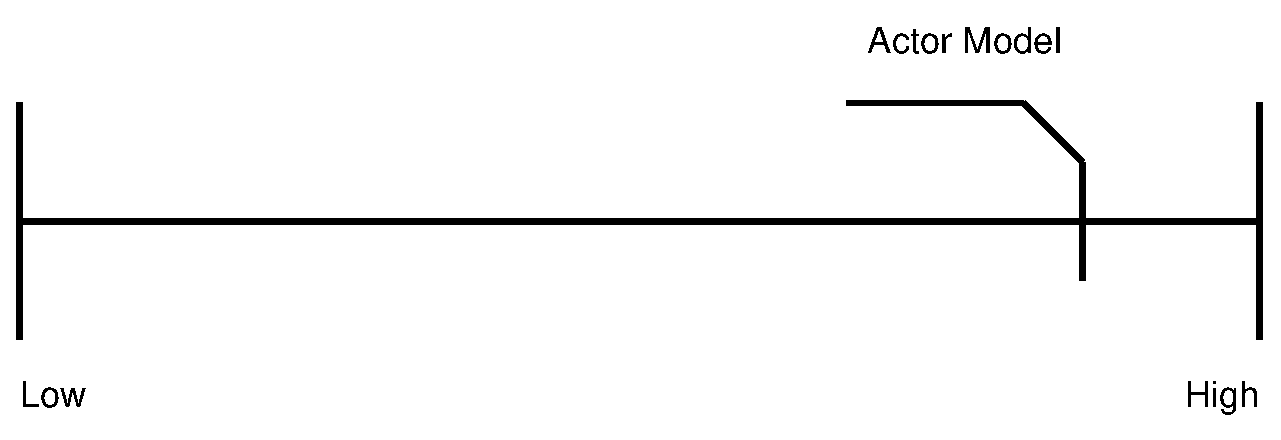
\includegraphics[width=0.9\textwidth]{\rootpath/worksheets/actor/figures/characteristics/actor_char_level_of_abstraction} 
 \caption{The actor model on the low - high level of abstraction spectrum}
\label{fig:actor_level_of_abstraction}
\end{figure}

\subsubsection{Expressivity}\label{sec:actor_expressivity}
Expressivity relates closely to the level of abstraction. The actor model ensures mutual exclusion for all state variables implicitly and let the programmer express programs through the abstraction of actors, without having to worry about the complications of the underlying threads. Furthermore, an actor only need the name of another actor to send it a message. The programmer does not have to worry about the complications in regards to communicating with another actor, such as the physical location of the actor and establishing a connection for sending the message to the actors mailbox. This location transparency enables simple distribution of actors on a cluster of machines. The Akka actor implementation enables the programmer to program the system on a single computer and distribute actors to a cluster of machines by modifying a config file.

However, the conceptual actor model does not provide constructs to prune non-determinism which means the programmer must build patterns for such coordination manually. This hurts the expressivity of the actor model, but most actor implementations typically have some useful coordination patterns, which reduces the impact on expressivity.

Based on these observations we have placed the expressivity in the high end of the spectrum, as shown on BLA\toby{indsæt ref}. We have not placed it on the highest expressivity as programmers may have to build patterns for communication manually.

%TL complications: explicitly start, stop and synchronize threads and choose explicitly which state variables should be ensured mutual exclusion.

\missingfigure{Høj expressivitiy - tæt på højst}

\begin{figure}[htbp]
\centering
 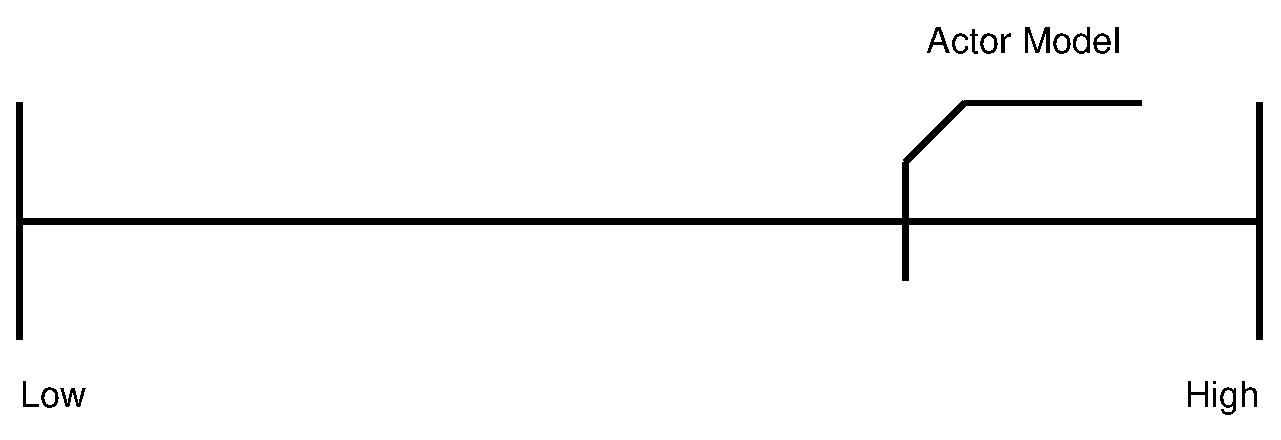
\includegraphics[width=0.9\textwidth]{\rootpath/worksheets/actor/figures/characteristics/actor_char_expressivity} 
 \caption{The actor model on the low - high level of expressivity spectrum}
\label{fig:actor_expressivity}
\end{figure}

\subsubsection{Writability evaluation}
The actor model allows the programmer to express concurrency solely through modelling of actor entities and the communication between them. The details and complications of threads, physical location of actors and connection management for sending and receiving messages are abstracted away from the programmer. Furthermore, as the actor model consider only isolated state and atomic processing of messages, it provides simple synchronization by design which avoids race conditions. Abstracting away these complications makes it simpler to write concurrent programs and has a positive influence on the writability. Additionally, the model enables a valuable environment for testing as each actor can be tested in isolation. This also has a positive effect on the writability and makes it simple have use a test-first implementation technique.

However, the notion of no shared state and asynchronous message passing can hurt the writability of the actor model initially as it requires a different mindset. In some situations a non-deterministic message order is not feasible and patterns for coordination between actor is needed. Such patterns does not exist in the conceptual actor model, but are often included in actor implementations which reduces the negative impact on writability. Additionally, the programmer must also take into account some problems only releated to the actor model such as proper message size and overflow of an actor mailbox, as discussed in \bsref{sec:actor_discussion}.

Based on the above observations and the evaluation of simplicity, orthogonality, level of abstraction and expressivity we place the actor model between the middle and high end of the writability spectrum, as shown in BLA\toby{indsæt figur}.

\missingfigure{mellem mid og høj}
\begin{figure}[htbp]
\centering
 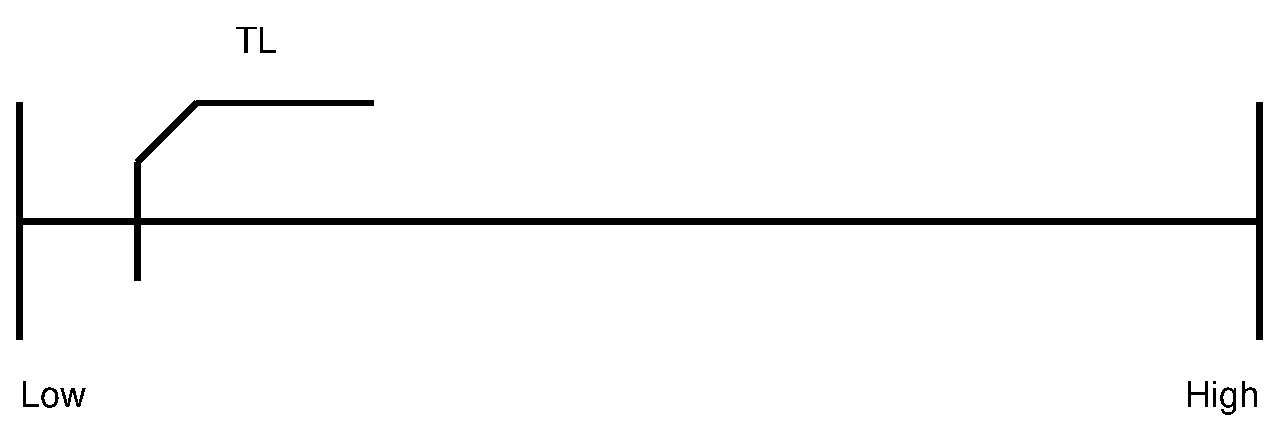
\includegraphics[width=0.9\textwidth]{\rootpath/worksheets/actor/figures/characteristics/actor_char_writability} 
 \caption{The actor model on the low - high level of writability spectrum}
\label{fig:actor_writability}
\end{figure}

%if the programmer does not adhere to the async nature of message passing and force blocking behaviour deadlocks can often occur.

\toby[i]{Til hvor vi skal vælge hvilken actor implementation vi vælger se ``Efficient Testing Of Actor Programs With Non-deterministic Behaviors - Samira Tasharofi'' for kort beskrivelse af Akka og at den ikke overholder nogle af properties}
\worksheetend
